\date{}
\title{}
\date{}
\begin{document}
\begin{frame}
    \titlepage
\end{frame}


\makeatletter
\newenvironment<>{btHighlight}[1][]
{\begin{onlyenv}#2\begingroup\tikzset{bt@Highlight@par/.style={#1}}\begin{lrbox}{\@tempboxa}}
{\end{lrbox}\bt@HL@box[bt@Highlight@par]{\@tempboxa}\endgroup\end{onlyenv}}

\newcommand<>\btHL[1][]{%
  \only#2{\begin{btHighlight}[#1]\bgroup\aftergroup\bt@HL@endenv}%
}
\def\bt@HL@endenv{%
  \end{btHighlight}%   
  \egroup %
}
\tikzset{
    btHLbox/.style={
        fill=red!30,outer sep=0pt,inner xsep=1pt, inner ysep=0pt, rounded corners=3pt
    },
}
\newcommand{\bt@HL@box}[2][]{%
  \tikz[#1]{%
    \pgfpathrectangle{\pgfpoint{1pt}{0pt}}{\pgfpoint{\wd #2}{\ht #2}}%
    \pgfusepath{use as bounding box}%
    \node[text width={},draw=none,anchor=base west, btHLbox, minimum height=\ht\strutbox+1pt,#1]{\raisebox{1pt}{\strut}\strut\usebox{#2}};
  }%
}

\lst@CCPutMacro
    \lst@ProcessOther {"2A}{%
      \lst@ttfamily 
         {\raisebox{2pt}{*}}% used with ttfamily
         {\raisebox{2pt}{*}}}% used with other fonts
    \@empty\z@\@empty

\lstdefinelanguage
   [x8664gas]{Assembler}     % add a "x64" dialect of Assembler
   [x86masm]{Assembler} % based on the "x86masm" dialect
   % with these extra keywords:
   {morekeywords={CDQE,CQO,CMPSQ,CMPXCHG16B,JRCXZ,LODSQ,MOVSXD,%
                  POPFQ,PUSHFQ,SCASQ,STOSQ,IRETQ,RDTSCP,SWAPGS,.TEXT,.STRING,.ASCIZ,%
                  BEQ,LW,SW,LB,SB,ADDIU,J,BEQZ,BNEZ,BNE,%
                  MOVUPD,MULPD,MOVSD,MULSD,%
                  SHLADD,MOV,CMP.LT,TBIT.NZ,BR.RET.SPTK.MANY,%
                  ADDQ,POPQ,PUSHQ,RRMOVQ,MRMOVQ,RMMOVQ,IRMOVQ,%
                  <-,LL,SC,ADDI,ADDL,VMOVDQA,ADDQ,CMPL,JB,JBE,MOVL,CLTQ,
                  MOVW,PUSHW,MOV,ADD,SUB,INT,PUSH,MOV,ADD,REP,MOVSB,%
                  TESTQ,CMPQ,MOVL,MOVQ,ADDQ,JMPQ,XORQ,%
                  LEAQ,LEAL,LEA,RETQ,RET,POPL,POPW,PUSHL,PUSHW,%
                  LEAW,%
                  SUBQ,SYSCALL,.ASCII,CALLQ,MOVSLQ,JMP,ANDQ,SHRQ,MOVB,INCQ,TESTL,XORL,%
                  SHRL,LEAL,SARL,SUBL,IMULL,IMULQ,MOVDQU,PADDD,XORL,%
                  MOVZBL,MOVZB,SHRB,SRAL,SHRL,ANDL,%
                  CMOVNS,SRAL,SRAQ,MOVZBW,MOVZBQ,%
                  PADDW,PADDQ,MODUPS,MOVAPD,%
                  MOVL,RET,.GLOBL,%
                  },
    deletekeywords={eax,ebx,sp,si,cx,di,ds,cs,es,fs,dx,ax,bx,al,esi,ebp,ecx,rip,eip,edx,edi,rdi,esp},
    morecomment=[l]{\#},
    morecomment=[l]{\/\/},
    morecomment=[s]{/*}{*/},
    sensitive=false,
    keepspaces=true} % et

\lstalias[]{myasm}[x8664gas]{Assembler}

\lstdefinelanguage{JavaScript}{
  keywords={typeof, new, true, false, catch, function, return, null, catch, switch, var, if, in, while, do, else, case, break},
  ndkeywords={class, export, boolean, throw, implements, import, this},
  sensitive=false,
  comment=[l]{//},
  morecomment=[s]{/*}{*/},
  morestring=[b]',
  morestring=[b]"
}

\newcommand{\keywordstyle}{\sourcecodeprolight\bfseries\color{blue!30!black}}
\newcommand{\stringstyle}{\color{blue!20!black}\ttfamily}

\lstset{
    language=C,
    basicstyle=\sourcecodepro\EmptyMapping,
    escapechar=`,
    keywordstyle=\keywordstyle\EmptyMapping,
    identifierstyle=\sourcecodepro\EmptyMapping,
    numberstyle=\small\color{black!70},
    commentstyle=\color{red!60!black}\ttfamily\itshape,
    stringstyle=\color{blue!20!black}\ttfamily,
    ndkeywordstyle=\bfseries\color{blue!30!black},
    upquote=true,
}



\lstdefinestyle{medium}{
    basicstyle=\sourcecodepro\EmptyMapping\fontsize{12}{13}\selectfont,
    keywordstyle=\sourcecodepro\EmptyMapping\fontsize{12}{13}\selectfont\keywordstyle,
}

\lstdefinestyle{small}{
    basicstyle=\sourcecodepro\EmptyMapping\small,
    keywordstyle=\sourcecodepro\EmptyMapping\small\keywordstyle,
}

\lstdefinestyle{smaller}{
    basicstyle=\sourcecodepro\EmptyMapping\fontsize{11}{12}\selectfont,
    keywordstyle=\sourcecodepro\EmptyMapping\fontsize{11}{12}\selectfont\keywordstyle,
}


\lstdefinestyle{script}{
    basicstyle=\sourcecodepro\EmptyMapping\scriptsize,
    keywordstyle=\sourcecodepro\EmptyMapping\scriptsize\bfseries,
}



\usetikzlibrary{circuits.logic.mux,matrix}
\makeatletter
\pgfdeclareshape{myregister}%
{
    \inheritsavedanchors[from=rectangle]
    \inheritanchorborder[from=rectangle]
    \inheritanchor[from=rectangle]{center}
    \inheritanchor[from=rectangle]{north}
    \inheritanchor[from=rectangle]{south}
    \inheritanchor[from=rectangle]{west}
    \inheritanchor[from=rectangle]{east}
    \inheritanchor[from=rectangle]{north east}
    \inheritanchor[from=rectangle]{north west}
    \inheritanchor[from=rectangle]{south east}
    \inheritanchor[from=rectangle]{south west}
    \inheritbackgroundpath[from=rectangle]
    \saveddimen{\halfbaselength}{%
         \pgf@x=0.5\wd\pgfnodeparttextbox
         % get xsep
         \pgfmathsetlength\pgf@xc{\pgfkeysvalueof{/pgf/inner xsep}}%
         \advance\pgf@x by \pgf@xc%
         % get \ht of textbox, add to baselength 
         \advance\pgf@x by \wd\pgfnodeparttextbox
         % get minimum width
         \pgfmathsetlength\pgf@xb{\pgfkeysvalueof{/pgf/minimum width}}%
         \divide\pgf@xb by 2
         \ifdim\pgf@x<\pgf@xb%
             % yes, too small. Enlarge...
             \pgf@x=\pgf@xb%
         \fi%
     }
    \backgroundpath{
        \pgfpathrectanglecorners{\southwest}{\northeast}
        \southwest \pgf@xa=\pgf@x \pgf@ya=\pgf@y 
        \pgf@yb=\pgf@ya
        \northeast \pgf@xb=\pgf@x %\pgf@yb=\pgf@y
        \pgf@xc = \pgf@xa
        \advance\pgf@xc by \halfbaselength
        \pgf@yc=\pgf@ya
        \advance\pgf@yc by \halfbaselength
        \pgfpathmoveto{\pgfpoint{\pgf@xa}{\pgf@ya}}
        \pgfpathlineto{\pgfpoint{\pgf@xc}{\pgf@yc}}
        \pgfpathlineto{\pgfpoint{\pgf@xb}{\pgf@yb}}
        \pgfpathclose
    }
}
\makeatother

\usetikzlibrary{arrows.meta}
\usetikzlibrary{fit}

\providecommand{\cpuset}{
\tikzset{
    box/.style={draw,very thick,align=center},
    cache/.style={box,fill=yellow!20,minimum width=2cm,minimum height=1.5cm},
    regfile/.style={box,fill=blue!20,minimum height=3cm,align=center},
    alu/.style={box,fill=violet!20,minimum height=1.5cm,minimum width=2cm},
    pc/.style={box,myregister,label={center:PC},minimum height=2cm,minimum width=.75cm,fill=yellow!30},
    connect/.style={draw,ultra thick,-Latex},
}
}
\providecommand{\cpucomponent}{
\node[pc] (pc) {};
\node[cache,anchor=west] (icache) at ([xshift=1cm]pc.east) {I\$};
\node[anchor=north,box,font=\small] (ilen) at ([yshift=-.25cm]icache.south) {+ instr\\len};
\node[regfile,anchor=north west] (regfile) at ([yshift=.5cm,xshift=1cm]icache.east) {register\\file};
\node[alu,anchor=west] (math) at ([xshift=1cm]regfile.east |- pc.east) {math};
\node[cache,anchor=west] (dcache) at ([xshift=1cm,yshift=-1cm]math.east) {D\$};
\node[anchor=north,font=\small] at ([yshift=-.1cm]regfile.north) {read};
\node[anchor=south east,font=\small] at ([yshift=.25cm]regfile.south east) {write};
}
\providecommand{\cpuconnect}{
\draw[connect] (pc) -- (icache);
\draw[connect] (pc.east) -- ++(0.5cm,0cm) |- (ilen.west);
\draw[connect] (ilen.east) -- ++(0.25cm,0cm) |- ([yshift=-1.5cm,xshift=-.5cm]pc.south west) |- (pc.west);
\coordinate (pre pc) at ([xshift=-.5cm,yshift=-1.5cm]pc.west);

\draw[connect] ([yshift=-.25cm]icache.north east) -- ([yshift=-.25cm]math.north west)
    coordinate[midway] (decode middle top) coordinate (math in top);
\draw[connect] ([yshift=-1cm]icache.north east) |- ([yshift=-1cm]icache.north east -| regfile.west) coordinate (regfile read in);

\draw[connect] ([yshift=-1cm]icache.north east -| regfile.east) coordinate (regfile read out) -- ([yshift=-1cm]math.north west) coordinate (reg to math);
\draw[connect] ([yshift=.5cm]math.south east) coordinate (math out 2) -- ([yshift=.5cm]math.south east -| dcache.west) coordinate (math to cache);
\draw[connect] ([yshift=-.5cm]math.north east) coordinate (math out 1) -- ([yshift=-.5cm,xshift=.75cm]math.north east -| dcache.east)
    |- ([xshift=.75cm,yshift=-.5cm]dcache.south east) -- ([yshift=-.5cm]dcache.south -| regfile.east);
\coordinate (memory top) at ([yshift=1cm]dcache.north);
\draw[connect] (dcache.east) -- ++(0.35cm,0cm) |- ([yshift=-.25cm]dcache.south -| regfile.east)
    coordinate (regfile write in);
\coordinate (regfile write in opposite) at (regfile write in -| regfile.west);
}

\providecommand{\stagestyles}{
\tikzset{
    stage/.style={draw,line width=1mm,opacity=0.7,fill opacity=0.2},
    fetch/.style={draw=yellow,fill=yellow},
    decode/.style={draw=orange,fill=orange},
    execute/.style={draw=green,fill=green},
    memory/.style={draw=blue,fill=blue},
    writeback/.style={draw=violet,fill=violet},
    fd reg/.style={draw=yellow!50!orange,fill=yellow!30!orange!30},
    de reg/.style={draw=orange!50!green,fill=orange!30!green!30},
    em reg/.style={draw=green!50!blue,fill=green!30!blue!30},
    mw reg/.style={draw=blue!50!violet,fill=blue!30!violet!30},
}
}
\providecommand{\stageboxes}{
    \node[stage,fetch,fit=(icache) (ilen),label={north:fetch}] (fetch) {};
    \node[stage,decode,fit=(regfile read in) (regfile read out) (decode middle top),label={north:decode}] (decode) {};
    \node[stage,execute,fit=(math in top) (math),label={north:execute}] (execute) {};
    \node[stage,memory,fit=(dcache) (memory top),label={north:memory}] (memory) {};
    \node[stage,writeback,fit=(regfile write in) (regfile write in opposite) (regfile.south),label={south:writeback}] (writeback) {};
}
\providecommand{\stageregs}{
    \node[draw,myregister,anchor=north,very thick,minimum width=0.1cm,minimum height=2cm,fd reg] (fd reg) at ([xshift=.25cm,yshift=0.25cm]fetch.north east) {};
    \node[draw,myregister,anchor=north,very thick,minimum width=0.1cm,minimum height=2cm,de reg] (de reg) at ([xshift=.25cm,yshift=0.25cm]decode.north east) {};
    \node[draw,myregister,anchor=north,very thick,minimum width=0.1cm,minimum height=3cm,em reg] (em reg) at ([xshift=.25cm,yshift=0.25cm]execute.north east) {};
    \node[draw,myregister,anchor=north,very thick,minimum width=0.1cm,minimum height=1cm,mw reg] (mw reg) at ([xshift=.5cm,yshift=0.25cm]writeback.north east) {};
}

\tikzset{
    matrix stages/.style={
        row 1 column 2/.append style={nodes={fill=yellow!20}},
        row 1 column 3/.append style={nodes={fill=orange!20}},
        row 1 column 4/.append style={nodes={fill=green!20}},
        row 1 column 5/.append style={nodes={fill=blue!20}},
        row 1 column 6/.append style={nodes={fill=violet!20}},
        nodes={text depth=0.2ex},
    },
    hiBox/.style={fill=red,opacity=0.2},
}



\begin{frame}{last time}
    \begin{itemize}
    \item pipeline idea
        \begin{itemize}
        \item instruction A in stage 3, while instruction B in stage 2, while instruction C in stage 3
        \end{itemize}
    \item register delays, uneven split limiting pipeline benefits
    \item control and data hazards
    \item stalling --- hardware inserted no-ops
    \item forwarding --- shortcut for value that hasn't made it to register file
    \end{itemize}
\end{frame}

\begin{frame}{some quiz notes (1)}
    \begin{itemize}
    \item some question writing issues on cryptography questions
    \vspace{.5cm}
    \item Q1B: As written: send duplicate message to forum A --- no problem, since no counters or similar. Meant to write ``same text they intended to go to forum B'' --- would be prevented because it would require forging MAC(k, forum name+msg).
    \item Q3A: Depends whether C can act as machine-in-the-middle (not specified in question)
    \item Q3E: Probably should have written `without B being able to detect it', but does not change answer
    \end{itemize}
\end{frame}

\begin{frame}[fragile]{some quiz notes (2)}
    \begin{itemize}
    \item on Q6E:
    \end{itemize}
\begin{Verbatim}
movq %r9, (%r10) // memory[r10] <- r9
movq %r10, %r11  // r11 <- r10
\end{Verbatim}
    \begin{itemize}
    \item first movq does not modify register \%r10 (or any registers)
    \item \ldots so no way for second movq to read `wrong version' of `\%r10'
    \end{itemize}
\end{frame}

\section{pipelining, con't}

\subsection{can't always forward: load-use}
\usetikzlibrary{positioning}
\begin{frame}[fragile,label=loadUse]{unsolved problem}
\lstset{
    language=myasm,
    morekeywords={mrmovq,irmovq,rmmovq,rrmovq},
    moredelim=**[is][\btHL<2|handout:0>]{~2~}{~end~},
    moredelim=**[is][\btHL<4|handout:0>]{~3~}{~end~},
}
\begin{tikzpicture}
\tikzset{
    forwardLine/.style={blue!60!black,thick,-Latex},
    hiForwardOn/.style={alt=#1{blue}{}},
    forwardLineB/.style={red,dashed,thick,-Latex},
    sepLine/.style={black!40,densely dotted},
};
\tikzset{fetch/.style={fill=yellow!15},decode/.style={fill=orange!15},execute/.style={fill=green!15},
memory/.style={fill=blue!15},writeback/.style={fill=violet!15}}
\providecommand{\fdemw}{ \& |[fetch]| F \& |[decode]| D \& |[execute]| E \& |[memory]| M \& |[writeback]| W}
\matrix[tight matrix no line,
        nodes={text width=.6cm,font=\tt,minimum height=.7cm,align=center},
        column 1/.style={nodes={text width=6cm,align=left}},
        row 3/.style={alt=<2->{opacity=0.25}{}},
        row 4/.style={visible on=<2->}] (tbl) {
|[align=right]| \normalfont\textit{cycle \#} \hspace{.5cm}
                                    \& 0 \& 1 \& 2 \& 3 \& 4 \& 5 \& 6 \& 7 \& 8 \\
\lstinline|movq 0(%rax), %rbx|   \fdemw \& ~ \& ~ \& ~ \& ~ \\
\lstinline|subq %rbx, %rcx|        \& ~ \fdemw \& ~ \& ~ \& ~ \\
\lstinline|subq %rbx, %rcx|        \& ~ \& |[fetch]| F \& |[decode]| D \& |[decode]| D \& |[execute]| E \& |[memory]| M \& |[writeback]| W \& ~ \& ~ \\
};
\foreach \x in {1,...,10} {
    \draw (tbl-1-\x.north east) -- (tbl-4-\x.south east);
}
\newcommand{\fwd}[4]{
    \pgfmathtruncatemacro{\idx}{#1+2}
    \draw[forwardLine,hiForwardOn=#4] ([xshift=-.15cm]tbl-#2-\idx.west) -- ([xshift=-.05cm]tbl-#3-\idx.west);
}
\newcommand{\fwdA}[4]{
    \pgfmathtruncatemacro{\idx}{#1+2}
    \draw[forwardLineB] ([xshift=-.15cm]tbl-#2-\idx.east) -- ([xshift=-.05cm]tbl-#3-\idx.east);
}

\newcommand{\fwdNo}[3]{
    \pgfmathtruncatemacro{\idx}{#1+2}
    \draw[forwardLineB] ([xshift=-.15cm]tbl-#2-\idx.west) -- ([xshift=-.05cm]tbl-#3-\idx.west);
}
\fwdNo{4}{2}{3}
\begin{visibleenv}<2->
    %\draw[thick,black!40] ([yshift=.1cm]tbl-3-1.west) -- ([yshift=-.1cm]tbl-3-10.east);
    \fwd{4}{2}{4}{<0|handout:0>}
\end{visibleenv}
\begin{visibleenv}<2->
    \node[draw,thick,red,fit=(tbl-4-4) (tbl-4-5)] {};
    \node [red,below=0cm of tbl-4-4] {stall};
\end{visibleenv}
\end{tikzpicture}
\begin{itemize}
    \item \textbf{combine} stalling and forwarding to resolve hazard
    \item assumption in diagram: hazard detected in \texttt{subq}'s decode stage
        \begin{itemize}
        \item (since easier than detecting it in fetch stage)
        \end{itemize}
\end{itemize}
\end{frame}


\subsubsection{can forward: load-to-store}
\begin{frame}[fragile,label=loadToStore]{solveable problem}
\lstset{
    language=myasm,
    morekeywords={mrmovq,irmovq,rmmovq,rrmovq},
    moredelim=**[is][\btHL<1-|handout:1->]{~begin~}{~end~},
    moredelim=**[is][\btHL<2|handout:0>]{~2~}{~end~},
    moredelim=**[is][\btHL<4|handout:0>]{~3~}{~end~},
}
\begin{tikzpicture}
\tikzset{
    forwardLine/.style={blue!60!black,thick,-Latex},
    hiForwardOn/.style={alt=#1{blue}{}},
    forwardLineB/.style={red,dashed,thick,-Latex},
    sepLine/.style={black!40,densely dotted},
}
\tikzset{fetch/.style={fill=yellow!15},decode/.style={fill=orange!15},execute/.style={fill=green!15},
memory/.style={fill=blue!15},writeback/.style={fill=violet!15}}
\providecommand{\fdemw}{ \& |[fetch]| F \& |[decode]| D \& |[execute]| E \& |[memory]| M \& |[writeback]| W}
\matrix[tight matrix no line,
        nodes={text width=.6cm,font=\tt,minimum height=.7cm,align=center},
        column 1/.style={nodes={text width=6cm,align=left}}] (tbl) {
|[align=right]| \normalfont\textit{cycle \#} \hspace{.5cm}
                                    \& 0 \& 1 \& 2 \& 3 \& 4 \& 5 \& 6 \& 7 \& 8 \\
\lstinline|movq 0(%rax), ~begin~%rbx~end~|   \fdemw \& ~ \& ~ \& ~ \& ~ \\
\lstinline|movq ~begin~%rbx~end~, 0(%rcx)|        \& ~ \fdemw \& ~ \& ~ \& ~ \\
};
\foreach \x in {1,...,10} {
   \draw (tbl-1-\x.north east) -- (tbl-3-\x.south east);
}
\newcommand{\fwd}[4]{
    \pgfmathtruncatemacro{\idx}{#1+2}
    \draw[forwardLine,hiForwardOn=#4] ([xshift=-.15cm]tbl-#2-\idx.west) -- ([xshift=-.05cm]tbl-#3-\idx.west);
}
\newcommand{\fwdA}[4]{
    \pgfmathtruncatemacro{\idx}{#1+2}
    \draw[forwardLineB] ([xshift=-.15cm]tbl-#2-\idx.east) -- ([xshift=-.05cm]tbl-#3-\idx.east);
}

\newcommand{\fwdNo}[3]{
    \pgfmathtruncatemacro{\idx}{#1+2}
    \draw[forwardLineB] ([xshift=-.15cm]tbl-#2-\idx.west) -- ([xshift=-.05cm]tbl-#3-\idx.west);
}
\fwd{4}{2}{3}{<0>}
\end{tikzpicture}
\end{frame}


\begin{frame}<1-2>[label=noForwardLoadUseCirc]{why can't we\ldots}
\begin{tikzpicture}
\cpuset
\cpucomponent
\cpuconnect
\stagestyles
\begin{pgfonlayer}{fg}
    \stageboxes
    \stageregs
    \draw[red,dotted,line width=.5mm,-Latex] ([xshift=.25cm]dcache.east) -- ++(0cm, 3cm) -| ([xshift=.725cm]regfile read out);
    \begin{visibleenv}<2->
    \draw[line width=0.75mm,red,-Latex] ([xshift=.5cm]math out 2) -- (dcache.east) -- ([xshift=.25cm]dcache.east)
        -- ++(0cm, 3cm) -| ([xshift=.725cm]regfile read out) -- ([xshift=0.125cm]math out 2);
    \end{visibleenv}
    \node[align=center,overlay,draw=red,ultra thick,fill=white,anchor=north] at ([xshift=-4cm,yshift=-1cm]dcache.south) {
        clock cycle needs to be long enough \\
        to go through data cache AND \\
        to go through math circuits! \\
        (which we were trying to avoid by putting them in separate stages)
    };
\end{pgfonlayer}
\end{tikzpicture}
\begin{tikzpicture}[remember picture,overlay]
        \node[font=\fontsize{64}{72}\selectfont,opacity=0.2,rotate=30] at (current page.center) { 
            INVALID
        };
\end{tikzpicture}
\end{frame}

% FIXME: show undoing instruction???



\subsection{dependency v hazard}

\begin{frame}{hazards versus dependencies}
    \begin{itemize}
        \item dependency --- X needs result of instruction Y?
            \begin{itemize}
                \item has potential for being messed up by pipeline
                \item (since part of X may run before Y finishes)
            \end{itemize}
        \item hazard --- will it not work in some pipeline?
            \begin{itemize}
                \item \myemph{before} extra work is done to ``resolve'' hazards
                \item multiple kinds: so far, \textit{data hazards}, \textit{control hazards}
            \end{itemize}
    \end{itemize}
\end{frame}


\begin{frame}[fragile,label=nonHazard]{ex.: dependencies and hazards (1)}
\begin{tikzpicture}
    \matrix[tight matrix no line,
            row sep=4mm,
            nodes={font=\tt,
                   text width=1.5cm,minimum width=2.5cm,text depth=.5ex},
            column 1/.style={nodes={text width=1.9cm,font=\tt\bfseries}},
    ] (instrs){
        addq \& \%rax, \& \%rbx \\
        subq \& \%rax, \& \%rcx \\
        irmovq \& \$100, \& \%rcx \\
        addq \& \%rcx, \& \%r10 \\
        addq \& \%rbx, \& \%r10 \\
    };
    \node[draw,below=.4cm of instrs,align=left] {
        where are dependencies? \\
        which are hazards in our pipeline? \\
        which are resolved wiht forwarding?
    };
    \tikzset{
        depHi/.style={draw,blue,thick,inner sep=0mm,inner xsep=-5mm,rounded corners},
        depLine/.style={blue,very thick,-Latex},
        hazHi/.style={draw,red,thick,inner sep=0mm,inner xsep=-5mm,rounded corners},
        hazLine/.style={red,very thick,-Latex},
    }
    \begin{visibleenv}<2->
        \node[fit=(instrs-1-3),depHi] (hiRBXWrite) {};
        \node[fit=(instrs-5-2),depHi] (hiRBXRead) {};
        \draw[depLine] (hiRBXWrite) -- (hiRBXRead);
    \end{visibleenv}
    \begin{visibleenv}<3->
        \node[fit=(instrs-3-3),hazHi] (hiRCXWrite) {};
        \node[fit=(instrs-4-2),hazHi] (hiRCXRead) {};
        \draw[hazLine] (hiRCXWrite) -- (hiRCXRead);
    \end{visibleenv}
    \begin{visibleenv}<4->
        \node[fit=(instrs-4-3),hazHi] (hiRTenWrite) {};
        \node[fit=(instrs-5-3),hazHi] (hiRTenRead) {};
        \draw[hazLine] (hiRTenWrite) -- (hiRTenRead);
    \end{visibleenv}
\end{tikzpicture}
\end{frame}


\subsection{with different pipeline?}
\begin{frame}[fragile,label=diffHaz]{pipeline with different hazards}
\lstset{
    language=myasm,
    style=small,
    morekeywords={mrmovq,irmovq,rmmovq,rrmovq,andq},
    moredelim=**[is][\btHL<1|handout:1>]{~1~}{~end~},
}
    \begin{itemize}
        \item example: 4-stage pipeline: fetch/decode/execute+memory/writeback
\begin{lstlisting}
                 // 4 stage  // 5 stage
addq %rax, ~1~%r8~end~   //          // W
subq %rax, %r9   // W        // M
xorq %rax, %r10  // EM       // E
andq ~1~%r8~end~,  %r11  // D        // D
\end{lstlisting}
        \item<2> addq/andq is hazard with 5-stage pipeline
        \item<2> addq/andq is \textbf{not} a hazard with 4-stage pipeline
        \item<3> \myemph<3>{more hazards with more pipeline stages}
    \end{itemize}
\end{frame}



\subsubsection{exercise}
\begin{frame}[fragile,label=diffHazEx]{exercise: different pipeline}
\lstset{
    language=myasm,
    morekeywords={mrmovq,irmovq,rmmovq,rrmovq,addq},
    moredelim=**[is][\btHL<2|handout:0>]{~2~}{~end~},
    moredelim=**[is][\btHL<4|handout:0>]{~3~}{~end~},
}
\begin{itemize}
\item split execute into two stages: F/D/E1/E2/M/W
\item result only available near end of second execute stage
\item where does forwarding, stalls occur?
\end{itemize}
\begin{tikzpicture}
\tikzset{
    forwardLine/.style={blue!60!black,thick,-Latex},
    hiForwardOn/.style={alt=#1{blue}{}},
    forwardLineB/.style={red,dashed,thick,-Latex},
    sepLine/.style={black!40,densely dotted},
};
\matrix[tight matrix no line,
        nodes={text width=.75cm,font=\tt,minimum height=.7cm,align=center},
        column 1/.style={nodes={text width=7cm,align=left}},
        ] (tbl) {
|[align=right]| \normalfont\textit{cycle \#} \hspace{.5cm}
                                 \& 0 \& 1 \& 2 \& 3 \& 4 \& 5 \& 6 \& 7 \& 8 \\
(1) \lstinline|addq %rcx, %r9|       \& F \& D \& E1\& E2\& M \& W \& ~ \& ~ \& ~ \\
(2) \lstinline|addq %r9, %rbx|       \& ~ \& F \& D \& D \& E1\& E2\& M \& W \& ~ \\
(3) \lstinline|addq %rax, %r9|       \& ~ \& ~ \& F \& F \& D \& E1\& E2\& M \& W  \\
(4) \lstinline|movq %r9, (%rbx)|   \& ~ \& ~ \& ~ \& F \& D \& E1\& E2\& M \& W  \\
(5) \lstinline|movq %rcx, %r9|     \& ~ \& ~ \& ~ \& ~ \& F \& D \& E1 \& E2 \& M \& W \\
};
\begin{visibleenv}<1|handout:1>
    \fill[white] (tbl-3-2.north west) rectangle (tbl-6-11.south east);
\end{visibleenv}
\newcommand{\fwd}[4]{
    \pgfmathtruncatemacro{\idx}{#1+2}
    \draw[forwardLine,hiForwardOn=#4] ([xshift=-.15cm]tbl-#2-\idx.west) -- ([xshift=-.05cm]tbl-#3-\idx.west);
}
\newcommand{\fwdA}[4]{
    \pgfmathtruncatemacro{\idx}{#1+2}
    \draw[forwardLineB] ([xshift=-.15cm]tbl-#2-\idx.east) -- ([xshift=-.05cm]tbl-#3-\idx.east);
}

\newcommand{\fwdNo}[3]{
    \pgfmathtruncatemacro{\idx}{#1+2}
    \draw[forwardLineB] ([xshift=-.15cm]tbl-#2-\idx.west) -- ([xshift=-.05cm]tbl-#3-\idx.west);
}
\foreach \x in {1,...,10} {
    \draw[dotted] (tbl-1-\x.north east) -- (tbl-6-\x.south east);
}
\end{tikzpicture}
\end{frame}

\begin{frame}[fragile,label=diffHazExSoln]{exercise: different pipeline}
\lstset{
    language=myasm,
    morekeywords={mrmovq,irmovq,rmmovq,rrmovq,addq},
    moredelim=**[is][\btHL<2|handout:0>]{~2~}{~end~},
    moredelim=**[is][\btHL<4|handout:0>]{~3~}{~end~},
}
\begin{itemize}
\item split execute into two stages: F/D/E1/E2/M/W
\end{itemize}
\begin{tikzpicture}
\tikzset{
    forwardLine/.style={blue!60!black,thick,-Latex},
    hiForwardOn/.style={alt=#1{blue}{}},
    forwardLineB/.style={red,dashed,thick,-Latex},
    sepLine/.style={black!40,densely dotted},
};
\matrix[tight matrix no line,
        nodes={text width=.75cm,font=\tt,minimum height=.7cm,align=center},
        column 1/.style={nodes={text width=5.2cm,align=left}},
        row 4/.style={nodes={visible on=<3-|handout:2>}},
        row 3/.style={nodes={alt=<1-2|handout:1>{}{opacity=0.2}}},
        row 6/.style={nodes={visible on=<3-|handout:2>}},
        row 5/.style={nodes={alt=<1-2|handout:1>{}{opacity=0.2}}},
        row 8/.style={nodes={visible on=<3-|handout:2>}},
        row 7/.style={nodes={alt=<1-2|handout:1>{}{opacity=0.2}}},
        row 9/.style={nodes={visible on=<5-|handout:1>}},
        row 10/.style={nodes={visible on=<1-|handout:1>}},
        row 11/.style={nodes={visible on=<1-|handout:1>}},
        ] (tbl) {
|[align=right]| \normalfont\textit{cycle \#} \hspace{.5cm}
                                 \& 0 \& 1 \& 2 \& 3 \& 4 \& 5 \& 6 \& 7 \& 8 \\
\lstinline|addq %rcx, %r9|       \& F \& D \& E1\& E2\& M \& W \& ~ \& ~ \& ~ \\
\lstinline|addq %r9, %rbx|       \& ~ \& F \& D \& E1\& E2\& M \& W \& ~ \& ~ \\
\lstinline|addq %r9, %rbx|       \& ~ \& F \& D \& D \& E1\& E2\& M \& W \& ~ \\
\lstinline|addq %rax, %r9|       \& ~ \& ~ \& F \& D \& E1\& E2\& M \& W \& ~ \\
\lstinline|addq %rax, %r9|       \& ~ \& ~ \& F \& F \& D \& E1\& E2\& M \& W  \\
\lstinline|movq %r9, (%rbx)|   \& ~ \& ~ \& ~ \& F \& D \& E1\& E2\& M \& W  \\
\lstinline|movq %r9, (%rbx)|   \& ~ \& ~ \& ~ \& ~ \& F \& D \& E1\& E2\& M \& W  \\
\lstinline|movq %rcx, %r9|     \& ~ \& ~ \& ~ \& ~ \& ~ \& F \& D \& E1 \& E2 \& M \& W \\
};
\begin{visibleenv}<1|handout:1>
    \fill[white] (tbl-3-2.north west) rectangle (tbl-8-11.south east);
\end{visibleenv}
\newcommand{\fwd}[4]{
    \pgfmathtruncatemacro{\idx}{#1+2}
    \draw[forwardLine,hiForwardOn=#4] ([xshift=-.15cm]tbl-#2-\idx.west) -- ([xshift=-.05cm]tbl-#3-\idx.west);
}
\newcommand{\fwdA}[4]{
    \pgfmathtruncatemacro{\idx}{#1+2}
    \draw[forwardLineB] ([xshift=-.15cm]tbl-#2-\idx.east) -- ([xshift=-.05cm]tbl-#3-\idx.east);
}

\newcommand{\fwdNo}[3]{
    \pgfmathtruncatemacro{\idx}{#1+2}
    \draw[forwardLineB] ([xshift=-.15cm]tbl-#2-\idx.west) -- ([xshift=-.05cm]tbl-#3-\idx.west);
}
\foreach \x in {1,...,10} {
    \draw[dotted] (tbl-1-\x.north east) -- (tbl-8-\x.south east);
}
\iftoggle{heldback}{}{
\begin{visibleenv}<2|handout:1>
    \fwdNo{3}{2}{3}
    \node[align=left,draw=red,fill=white,anchor=north] at (tbl-4-5.south) {
        r9 not available yet --- can't forward here \\
        so try stalling in addq's decode\ldots
    };
\end{visibleenv}
\begin{visibleenv}<3-|handout:2>
    \fwd{4}{2}{4}{<3|handout:0>}
\end{visibleenv}
\begin{visibleenv}<3>
    \node[draw=red,fill=white,anchor=north] at (tbl-4-5.south) {
        after stalling once, now we can forward
    };
\end{visibleenv}
\begin{visibleenv}<4-|handout:2>
    \fwd{5}{2}{6}{<4|handout:0>}
\end{visibleenv}
\begin{visibleenv}<5-|handout:2>
    \fwd{6}{4}{8}{<5|handout:0>}
    \fwd{8}{6}{8}{<5|handout:0>}
\end{visibleenv}
}
\end{tikzpicture}
\end{frame}


\section{OOO}

\subsection{introduction}

\subsection{multiple issue}
\usetikzlibrary{arrows.meta,matrix}

\begin{frame}[fragile,label=multiIssueIntro]{beyond pipelining: multiple issue}
    \begin{itemize}
    \item start \myemph{more than one instruction/cycle}
    \item multiple parallel pipelines; many-input/output register file
    \item \myemph{hazard handling much more complex}
    \end{itemize}
\begin{tikzpicture}
\tikzset{
    forwardLine/.style={blue!60!black,thick,-Latex},
    hiForwardOn/.style={alt=#1{blue}{}},
    forwardLineB/.style={red,dashed,thick,-Latex},
    sepLine/.style={black!40,densely dotted},
};
    \tikzset{fetch/.style={fill=yellow!15},decode/.style={fill=orange!15},execute/.style={fill=green!15},
    memory/.style={fill=blue!15},writeback/.style={fill=violet!15},commit/.style={fill=magenta!15}}
\newcommand{\fdemw}{ \& |[fetch]| F \& |[decode]| D \& |[execute]| E \& |[memory]| M \& |[writeback]| W}
\newcommand{\fdem}{ \& |[fetch]| F \& |[decode]| D \& |[execute]| E \& |[memory]| M }
\newcommand{\m}{ \& |[memory]| M }
\newcommand{\w}{ \& |[writeback]| W }
\newcommand{\dec}{ \& |[decode]| D } % conflicts with existing \d macro
\newcommand{\e}{ \& |[execute]| E }
\newcommand{\f}{ \& |[fetch]| F }
\matrix[tight matrix no line,
        nodes={text width=.75cm,font=\tt,minimum height=.7cm,align=center},
        column 1/.style={nodes={text width=5.2cm,align=left}},
        ] (tbl) {
|[align=right]| \normalfont\textit{cycle \#} \hspace{.5cm}
                                 \& 0 \& 1 \& 2 \& 3 \& 4 \& 5 \& 6 \& 7 \& 8 \\
\lstinline|addq %r8, %r9|       \fdemw \& ~ \& ~ \& ~ \\
\lstinline|subq %r10, %r11|     \fdemw \& ~ \& ~ \& ~ \\
\lstinline|xorq %r9, %r11|      \& ~  \fdemw \& ~ \& ~ \& ~ \\
\lstinline|subq %r10, %rbx|     \& ~  \fdemw \& ~ \& ~ \& ~ \\
\ldots \\
};
\newcommand{\fwd}[4]{
    \pgfmathtruncatemacro{\idx}{#1+2}
    \draw[forwardLine,hiForwardOn=#4] ([xshift=-.15cm]tbl-#2-\idx.west) -- ([xshift=-.05cm]tbl-#3-\idx.west);
}
\newcommand{\fwdO}[4]{
    \pgfmathtruncatemacro{\idx}{#1+2}
    \draw[forwardLine,hiForwardOn=#4] ([xshift=-.05cm]tbl-#2-\idx.west) -- ([xshift=+.05cm]tbl-#3-\idx.west);
}
\newcommand{\fwdA}[4]{
    \pgfmathtruncatemacro{\idx}{#1+2}
    \draw[forwardLineB] ([xshift=-.15cm]tbl-#2-\idx.east) -- ([xshift=-.05cm]tbl-#3-\idx.east);
}

\newcommand{\fwdNo}[3]{
    \pgfmathtruncatemacro{\idx}{#1+2}
    \draw[forwardLineB] ([xshift=-.15cm]tbl-#2-\idx.west) -- ([xshift=-.05cm]tbl-#3-\idx.west);
}
\fwdO{3}{2}{4}{<0>}
%\fwd{3}{3}{5}{<0>}
\fwd{3}{3}{4}{<0>}
\end{tikzpicture}
\end{frame}



\subsection{out-of-order issue}
\usetikzlibrary{arrows.meta,matrix}

\begin{frame}[fragile,label=oooIntro]{beyond pipelining: out-of-order}
    \begin{itemize}
    \item find \myemph{later instructions to do} instead of stalling
    \item lists of available instructions in pipeline registers
        \begin{itemize}
        \item take any instruction with available values
        \end{itemize}
    \item provide \myemph{illusion that work is still done in order}
        \begin{itemize}
        \item much more complicated hazard handling logic
        \end{itemize}
    \end{itemize}
\begin{tikzpicture}
\tikzset{
    forwardLine/.style={blue!60!black,thick,-Latex},
    hiForwardOn/.style={alt=#1{blue}{}},
    forwardLineB/.style={red,dashed,thick,-Latex},
    sepLine/.style={black!40,densely dotted},
};
    \tikzset{fetch/.style={fill=yellow!15},decode/.style={fill=orange!15},execute/.style={fill=green!15},
    memory/.style={fill=blue!15},writeback/.style={fill=violet!15},commit/.style={fill=magenta!20}}
\newcommand{\fdemw}{ \& |[fetch]| F \& |[decode]| D \& |[execute]| E \& |[memory]| M \& |[writeback]| W}
\newcommand{\fdem}{ \& |[fetch]| F \& |[decode]| D \& |[execute]| E \& |[memory]| M }
\newcommand{\m}{ \& |[memory]| M }
\newcommand{\w}{ \& |[writeback]| W }
\newcommand{\cmt}{ \& |[commit]| C }
\newcommand{\dec}{ \& |[decode]| D } % conflicts with existing \d macro
\newcommand{\e}{ \& |[execute]| E }
\newcommand{\f}{ \& |[fetch]| F }
\matrix[tight matrix no line,
        nodes={text width=.75cm,font=\tt,minimum height=.7cm,align=center},
        column 1/.style={nodes={text width=5.8cm,align=left}},
        ] (tbl) {
|[align=right]| \normalfont\textit{cycle \#} \hspace{.5cm}
                                 \& 0 \& 1 \& 2 \& 3 \& 4 \& 5 \& 6 \& 7 \& 8 \& 9 \& 10 \& 11\\
    \lstinline|mrmovq 0(%rbx), %r8| \fdem                  \m   \m   \w \cmt\\
    \lstinline|subq %r8, %r9|       \& ~   \f \& ~ \& ~ \& ~  \& ~  \dec \e \w \cmt\\
    \lstinline|addq %r10, %r11|     \& ~ \& ~    \f   \dec  \e  \w \& ~ \& ~ \& ~ \& \cmt \\
    \lstinline|xorq %r12, %r13|     \& ~ \& ~ \& ~     \f   \dec \e \w  \& ~ \& ~ \& ~ \& \cmt \\
\ldots \\
};
\newcommand{\fwd}[4]{
    \pgfmathtruncatemacro{\idx}{#1+2}
    \draw[forwardLine,hiForwardOn=#4] ([xshift=-.15cm]tbl-#2-\idx.west) -- ([xshift=-.05cm]tbl-#3-\idx.west);
}
\newcommand{\fwdO}[4]{
    \pgfmathtruncatemacro{\idx}{#1+2}
    \draw[forwardLine,hiForwardOn=#4] ([xshift=-.05cm]tbl-#2-\idx.west) -- ([xshift=+.05cm]tbl-#3-\idx.west);
}
\newcommand{\fwdA}[4]{
    \pgfmathtruncatemacro{\idx}{#1+2}
    \draw[forwardLineB] ([xshift=-.15cm]tbl-#2-\idx.east) -- ([xshift=-.05cm]tbl-#3-\idx.east);
}

\newcommand{\fwdNo}[3]{
    \pgfmathtruncatemacro{\idx}{#1+2}
    \draw[forwardLineB] ([xshift=-.15cm]tbl-#2-\idx.west) -- ([xshift=-.05cm]tbl-#3-\idx.west);
}
\end{tikzpicture}
\end{frame}


\subsection{real CPUs}
\begin{frame}{interlude: real CPUs}
    \begin{itemize}
    \item modern CPUs:
    \vspace{.5cm}
    \item execute \myemph{multiple instructions at once}
    \item execute instructions \myemph{out of order} --- whenever \myemph{values available}
    \end{itemize}
\end{frame}


\subsection{complex hazards examples}
\usetikzlibrary{arrows.meta,matrix}

\begin{frame}<1>[fragile,label=oooHazardIndex]{out-of-order and hazards}
    \begin{itemize}
    \item out-of-order execution makes hazards harder to handle
    \vspace{.5cm}
    \item problems for forwarding:
    \begin{itemize}
        \item \myemph<3>{value in last stage may not be most up-to-date}
        \item older value may be written back before newer value?
    \end{itemize}
    \item problems for branch prediction:
    \begin{itemize}
        \item mispredicted instructions may complete execution before squashing
    \end{itemize}
    \item which instructions to dispatch?
        \begin{itemize}
        \item how to quickly find instructions that are ready?
        \end{itemize}
    \end{itemize}
\end{frame}

\againframe<2>{oooHazardIndex}

\begin{frame}[fragile,label=rawExamples1]{read-after-write examples (1)}
\lstset{
    language=myasm,
    morekeywords={mrmovq,irmovq,rmmovq,rrmovq,addq},
    moredelim=**[is][\btHL<2|handout:0>]{~2~}{~end~},
    moredelim=**[is][\btHL<4|handout:0>]{~3~}{~end~},
}
\tikzset{
    forwardLine/.style={blue!60!black,thick,-Latex},
    %hiForwardOn/.style={alt=#1{blue}{}},
    hiForwardOn/.style={},
    forwardLineB/.style={red,dashed,thick,-Latex},
    sepLine/.style={black!40,densely dotted},
}
    \tikzset{fetch/.style={fill=yellow!15},decode/.style={fill=orange!15},execute/.style={fill=green!15},
    memory/.style={fill=blue!15},writeback/.style={fill=violet!15},commit/.style={fill=magenta!20}}
\newcommand{\fdemw}{ \& |[fetch]| F \& |[decode]| D \& |[execute]| E \& |[memory]| M \& |[writeback]| W}
\newcommand{\F}{ \& |[fetch]| F}
\newcommand{\fd}{ \& |[fetch]| F \& |[decode]| D}
\newcommand{\demw}{ \& |[decode]| D \& |[execute]| E \& |[memory]| M \& |[writeback]| W}
\newcommand{\emw}{ \& |[execute]| E \& |[memory]| M \& |[writeback]| W}
\newcommand{\mw}{  \& |[memory]| M \& |[writeback]| W}
\newcommand{\mem}{  \& |[memory]| M}
\newcommand{\cmt}{ \& |[commit]| C }
\begin{tikzpicture}
\matrix[tight matrix no line,
        nodes={text width=.6cm,font=\tt,minimum height=.7cm,align=center},
        column 1/.style={nodes={text width=6cm,align=left}}] (tbl) {
|[align=right]| \normalfont\textit{cycle \#} \hspace{.5cm}
                                    \& 0 \& 1 \& 2 \& 3 \& 4 \& 5 \& 6 \& 7 \& 8 \\
\lstinline|addq %r10, ~2~%r8~end~|   \fdemw \& ~ \& ~ \& ~ \& ~ \\
\lstinline|addq %r11, ~2~%r8~end~|   \& ~ \fdemw \\
\lstinline|addq %r12, ~2~%r8~end~|   \& ~ \& ~ \fdemw \& ~ \& ~ \\
};
\newcommand{\fwd}[4]{
    \pgfmathtruncatemacro{\idx}{#1+2}
    \draw[forwardLine,hiForwardOn=#4] ([xshift=-.15cm]tbl-#2-\idx.west) -- ([xshift=-.05cm]tbl-#3-\idx.west);
}
\fwd{4}{3}{4}{<0>}
\foreach \x in {1,...,10} {
    \draw (tbl-1-\x.north east) -- (tbl-4-\x.south east);
}
\end{tikzpicture}
\hrule
\begin{onlyenv}<1>
normal pipeline: two options for \%r8? \\
choose the one from \textit{earliest stage} \\
because it's from the most recent instruction
\end{onlyenv}
\begin{onlyenv}<2->
\begin{tikzpicture}
\matrix[tight matrix no line,
        nodes={text width=.6cm,font=\tt,minimum height=.7cm,align=center},
        column 1/.style={nodes={text width=6cm,align=left}},
        row 3/.append style={nodes={opacity=0.4}},
        ] (tbl) {
|[align=right]| \normalfont\textit{cycle \#} \hspace{.5cm}
                                    \& 0 \& 1 \& 2 \& 3 \& 4 \& 5 \& 6 \& 7 \& 8 \\
\lstinline|addq %r10, ~2~%r8~end~|   \F \& ~ \& ~ \& ~ \&\demw \& ~ \& ~ \& ~ \& ~ \\
\lstinline|movq %r8, (%rax)|        \& \F \&  ~ \& ~ \& ~ \&\demw \& ~ \& ~ \& ~ \& ~ \\
\lstinline|movq $100, ~2~%r8~end~|   \& ~  \& \fdemw \\
\lstinline|addq %r13, ~2~%r8~end~|   \& ~ \& ~  \& \F \& ~ \& \demw \& ~ \& ~ \\
};
\newcommand{\fwdB}[4]{
    \pgfmathtruncatemacro{\idx}{#1+2}
    \draw[forwardLineB,hiForwardOn=#4] ([xshift=-.15cm]tbl-#2-\idx.west) -- ([xshift=-.05cm]tbl-#3-\idx.west);
}
\fwdB{7}{2}{5}{<0>}
\end{tikzpicture}
\begin{tikzpicture}[overlay,remember picture]
\node[align=left,draw=red,very thick,fill=white,anchor=north] at ([yshift=-1cm]current page.north) {
out-of-order execution: \\
\%r8 from earliest stage might be from \textit{delayed instruction} \\
can't use same forwarding logic
};
\end{tikzpicture}
\end{onlyenv}
\end{frame}

\begin{frame}{register version tracking}
\begin{itemize}
\item goal: track \myemph{different versions of registers}
\item out-of-order execution: may compute versions at different times
\item only forward the \myemph{correct version}
\vspace{.5cm}
\item strategy for doing this: preprocess instructions represent version info
\item makes forwarding, etc. lookup easier
\end{itemize}
\end{frame}

\begin{frame}[fragile,label=rawRewriting1]{rewriting hazard examples (1)}
\begin{tabular}{l|l}
\texttt{addq \%r10, \%r8} &
\texttt{addq \%r10, \%r8\textsubscript{v1} $\rightarrow$ \%r8\textsubscript{v2}} \\
\texttt{addq \%r11, \%r8} &
\texttt{addq \%r11, \%r8\textsubscript{v2} $\rightarrow$ \%r8\textsubscript{v3}} \\
\texttt{addq \%r12, \%r8} &
\texttt{addq \%r12, \%r8\textsubscript{v3} $\rightarrow$ \%r8\textsubscript{v4}} \\
\end{tabular}
\hrule
\begin{itemize}
\item read different version than the one written
    \begin{itemize}
    \item represent with three argument psuedo-instructions
    \end{itemize}
\item forwarding a value? must match version \textit{exactly}
\vspace{.5cm}
\item for now: version numbers
\item later: something simpler to implement
\end{itemize}
\end{frame}


\begin{frame}[fragile,label=wawExamples]{write-after-write example}
\lstset{
    language=myasm,
    morekeywords={mrmovq,irmovq,rmmovq,rrmovq,addq},
    moredelim=**[is][\btHL<2|handout:0>]{~2~}{~end~},
    moredelim=**[is][\btHL<4|handout:0>]{~3~}{~end~},
}
\tikzset{
    forwardLine/.style={blue!60!black,thick,-Latex},
    %hiForwardOn/.style={alt=#1{blue}{}},
    hiForwardOn/.style={},
    forwardLineB/.style={red,dashed,thick,-Latex},
    sepLine/.style={black!40,densely dotted},
}
    \tikzset{fetch/.style={fill=yellow!15},decode/.style={fill=orange!15},execute/.style={fill=green!15},
    memory/.style={fill=blue!15},writeback/.style={fill=violet!15},commit/.style={fill=magenta!20}}
\newcommand{\fdemw}{ \& |[fetch]| F \& |[decode]| D \& |[execute]| E \& |[memory]| M \& |[writeback]| W}
\newcommand{\fdem}{ \& |[fetch]| F \& |[decode]| D \& |[execute]| E \& |[memory]| M }
\newcommand{\F}{ \& |[fetch]| F}
\newcommand{\fd}{ \& |[fetch]| F \& |[decode]| D}
\newcommand{\demw}{ \& |[decode]| D \& |[execute]| E \& |[memory]| M \& |[writeback]| W}
\newcommand{\dem}{ \& |[decode]| D \& |[execute]| E \& |[memory]| M}
\newcommand{\emw}{ \& |[execute]| E \& |[memory]| M \& |[writeback]| W}
\newcommand{\mw}{  \& |[memory]| M \& |[writeback]| W}
\newcommand{\mem}{  \& |[memory]| M}
\newcommand{\cmt}{ \& |[commit]| C }
\begin{tikzpicture}
\matrix[tight matrix no line,
        nodes={text width=.6cm,font=\tt,minimum height=.7cm,align=center},
        column 1/.style={nodes={text width=6cm,align=left}},
        row 3/.append style={nodes={alt=<1-2>{opacity=0.4}}},
        row 5/.append style={nodes={alt=<1-2>{opacity=0.4}}},
        ] (tbl) {
|[align=right]| \normalfont\textit{cycle \#} \hspace{.5cm}
                                    \& 0 \& 1 \& 2 \& 3 \& 4 \& 5 \& 6 \& 7 \& 8 \\
\lstinline|addq %r10, ~2~%r8~end~|   \F \& ~ \& ~ \& ~ \&\dem \& |[writeback,draw=red,very thick]| W \& ~ \& ~ \& ~ \& ~ \\
\lstinline|movq ~3~%r8~end~, (%rax)|        \F \& ~ \& ~ \& ~ \& ~ \& ~ \& ~ \& ~ \&\demw \& ~ \& ~ \& ~ \& ~ \\
\lstinline|movq %r11, ~2~%r8~end~|   \& ~ \fdemw \\
\lstinline|movq ~3~%r8~end~, 8(%rax)|     \& ~ \F \& ~ \& ~ \& ~ \& ~ \& ~ \demw \& ~ \& ~ \& ~ \& ~ \\
    \lstinline|movq $100, ~2~%r8~end~|   \& \& \fdem \& |[writeback,draw=red,very thick]| W  \\
\lstinline|addq %r13, ~2~%r8~end~|   \& ~ \& ~  \F \& ~ \& ~ \& ~ \& ~ \& ~ \& \demw \& ~ \& ~ \\
};
\newcommand{\fwdB}[4]{
    \pgfmathtruncatemacro{\idx}{#1+2}
    \draw[forwardLineB,hiForwardOn=#4] ([xshift=-.15cm]tbl-#2-\idx.west) -- ([xshift=-.05cm]tbl-#3-\idx.west);
}
\end{tikzpicture}
\begin{tikzpicture}[overlay,remember picture]
\begin{visibleenv}<2>
\node[align=left,draw=red,very thick,fill=white,anchor=south] at ([yshift=.5cm]current page.south) {
out-of-order execution: \\
if we don't do something, newest value could be overwritten!
};
\end{visibleenv}
\begin{visibleenv}<3>
\node[align=left,draw=red,very thick,fill=white,anchor=south] at ([yshift=.5cm]current page.south) {
two instructions that haven't been started \\
could need \textit{different versions} of \%r8!
};
\end{visibleenv}
\end{tikzpicture}
\end{frame}

\begin{frame}{keeping multiple versions}
    \begin{itemize}
    \item for write-after-write problem: need to keep copies of multiple versions
        \begin{itemize}
        \item both the new version and the old version needed by delayed instructions
        \end{itemize}
    \item for read-after-write problem: need to distinguish different versions
    \item solution: \myemph{have lots of extra registers}
    \item \myemph{\ldots and assign each version a new `real' register}
    \vspace{.5cm}
    \item called \myemph{register renaming}
    \end{itemize}
\end{frame}

\begin{frame}{register renaming}
    \begin{itemize}
    \item rename \textit{architectural registers} to \textit{physical registers}
    \item different physical register for each version of architectural
    \item track which physical registers are ready
    \item compare physical register numbers to do forwarding
    \end{itemize}
\end{frame}
 %FIXME

\subsection{superscalar overall design}
% FIXME: https://people.eecs.berkeley.edu/~krste/papers/BROOM-IEEEMicro2019.pdf
\usetikzlibrary{arrows.meta,calc,chains,shapes.multipart}

\begin{frame}<0>[fragile,label=oooPipe]{an OOO pipeline}
\begin{tikzpicture}
\tikzset{
    every node/.style={font=\fontsize{8.5}{9.5}\selectfont},
    every label/.style={font=\fontsize{8.5}{9.5}\selectfont,align=center,overlay},
    node distance=4mm,
    >=Latex,
    iqueue/.style={very thick,align=center,draw,rectangle split,rectangle split horizontal,rectangle split parts=3,
        inner sep=.25mm,minimum height=2.5cm,minimum width=2cm},
    cache/.style={align=center,draw,very thick,minimum height=1cm,
        inner sep=.25mm,minimum width=1cm},
    register/.style={fill=white,myregister,draw,thick,minimum height=5cm,yshift=-1cm,inner sep=0mm,minimum width=2mm},
    register short/.style={myregister,draw,thick,minimum height=3cm,yshift=0cm,inner sep=0mm,minimum width=2mm},
    register very short/.style={fill=white,myregister,draw,thick,minimum height=1cm,yshift=0cm,inner sep=0mm,minimum width=2mm},
    compute/.style={minimum height=3cm,rounded corners,draw,align=center,very thick,inner sep=.5mm},
    compute short/.style={minimum height=2cm,rounded corners,draw,align=center,very thick,inner sep=.5mm},
    compute very short/.style={minimum height=1cm,rounded corners,draw,align=center,very thick,inner sep=.5mm,
        font=\fontsize{8}{9}\selectfont},
    connect/.style={very thick,-{Latex[length=2mm]},black!70},
    connect both/.style={very thick,{Latex[length=2mm]}-{Latex[length=2mm]},black!70},
    hi on/.style={alt=<#1>{fill=red!20,draw=red}},
    predict/.style={hi on=2,hi on=15},
    rename/.style={hi on=3,hi on=4,hi on=13},
    issue/.style={hi on=5,hi on=11},
    regread/.style={hi on=6},
    execute/.style={hi on=7,hi on=12},
    writeback/.style={hi on=8},
    commit/.style={hi on=9,hi on=10,hi on=14,hi on=16},
}
\coordinate (main start) at (0,0);
\coordinate (low start) at (0, -3);
\coordinate (high start) at (0, 2);
\begin{scope}[start chain=going right]
\coordinate[on chain] (pc loc) at (main start);
\node[register short,anchor=center] (pc) at (pc loc) {};
\begin{scope}[node distance=6mm]
\node[cache,on chain,label={center:instr.\\cache}] (icache){};
\end{scope}
\node[compute short,anchor=center,predict] (bpEarly) at (icache.south |- low start) {branch\\predict};
\coordinate[on chain] (fetch 1 reg loc);
\node[register] (fetch 1 reg) at (fetch 1 reg loc) {};
\node[compute,on chain] (decode) {decode};
\node[compute short,anchor=center,predict] (bpLate) at (decode.south |- low start) {more\\branch\\predict};
\coordinate[on chain] (decode 1 reg loc);
\node[register] (decode 1 reg) at (decode 1 reg loc) {};
\node[compute,on chain,rename] (rename) {rename\\and\\dispatch};
\coordinate[on chain] (rename 1 reg loc);
\node[register] (rename 1 reg) at (rename 1 reg loc) {};
\node[issue,iqueue,on chain,label={north:instr.\\queue(s)}] (iqueue) {};
\begin{scope}[node distance=0.0cm]
\coordinate[on chain] (iqueue reg loc);
\end{scope}
%\node[register] (iqueue reg) at (iqueue reg loc) {};
\node[compute,on chain,regread] (regread) {issue \\ and \\ register \\ read \\ or \\ forward};
\node[cache,anchor=north,label={center:register\\file}] (regfile) at ([yshift=-.5cm]regread.south) {};
\node[cache,anchor=east,issue] (regready) at ([xshift=.025cm]regfile.west) {reg.\\ready\\info};
\draw[connect both] (regready.north) -- ++(0cm, .25cm) -| (regread.south);
\coordinate[on chain] (post read reg loc);
\node[register] (post read reg) at (post read reg loc) {};
\begin{scope}[node distance=0.7cm]
\coordinate[on chain] (execute loc);
\end{scope}
\begin{scope}[every node/.style={execute}]
\node[compute very short] (alu 1) at ([yshift=1cm]execute loc) {ALU\\1};
\node[compute very short] (alu 2) at ([yshift=-0.3cm]execute loc) {ALU\\2};
\node[compute very short] (alu 3a) at ([yshift=-1.7cm]execute loc) {ALU\\3\\pt 1};
\node[register very short,anchor=west] (alu 3a reg) at ([xshift=.1cm]alu 3a.east) {};
\node[compute very short,anchor=west] (alu 3b) at ([xshift=.1cm]alu 3a reg.east) {ALU\\3\\pt 2};
\node[compute very short] (loadstore) at ([yshift=-3cm]execute loc) {load\\store};
\end{scope}
\begin{scope}[node distance=1.9cm]
\coordinate[on chain] (prewriteback reg loc);
\end{scope}
\node[register] (prewriteback reg) at (prewriteback reg loc) {};
\node[compute,on chain,writeback] (wb) {write\\back};
\coordinate[on chain] (postwriteback reg loc);
\node[register] (postwriteback reg) at (postwriteback reg loc) {};
\node[compute,on chain,commit] (commit) {commit};
\end{scope}
\draw[connect] (pc.east) -- (icache.west);
\draw[connect] (pc.east) -- ++(1.5mm,0mm) |- (bpEarly.west);
\begin{pgfonlayer}{bg}
\draw[connect] (icache.east) -- (decode.west);
\draw[connect] (bpEarly) -- (bpLate);
\draw[connect] (bpEarly.south) -- ++(0mm,-1.5mm) -| ([xshift=-3mm]pc.west) -- (pc);
\draw[connect] (bpLate.south) -- ++(0mm,-1.5mm) -| ([xshift=-3mm]pc.west) -- (pc);
\draw[connect] (decode.south) -- (bpLate);
\draw[connect] (decode) -- (rename);
\draw[connect] (rename) -- (iqueue);
\draw[connect] (iqueue) -- (regread);
\draw[connect] (regread.east |- alu 1.east) -- (alu 1);
\draw[connect] (regread.east |- alu 2.east) -- (alu 2);
\draw[connect] (regread.east |- alu 2.east) -- ++(1mm,0mm) |- (alu 3a.west);
\draw[connect] (regread.east |- alu 2.east) -- ++(1mm,0mm) |- (loadstore.west);
\draw[connect] (alu 1) -- (alu 1 -| prewriteback reg.west);
\draw[connect] (alu 2) -- (alu 2 -| prewriteback reg.west);
\draw[connect] (alu 3b) -- (alu 3b -| prewriteback reg.west);
\draw[connect] (loadstore) -- (loadstore -| prewriteback reg.west);
\draw[connect] (prewriteback reg.east |- wb.west) -- (wb);
\draw[connect] (wb) -- (commit);
\draw[connect both] (regread) -- (regfile);
\draw[connect] (wb.south) -- ++(0mm,-2.25cm) -| (regfile.south);
\draw[connect] (wb.south) -- ++(0mm,-2.25cm) -| (regready.south);
\node[commit,cache,anchor=north,label={center:reorder\\buffer}] (rob) at ([yshift=-1cm]commit.south) {};
\draw[connect both] (commit) -- (rob);
\draw[connect both] (rename.south) -- ++(0mm,-2.5cm) -| (rob.south);
\end{pgfonlayer}
\tikzset{
    box/.style={at={(7.5,-4.3)},anchor=north,draw=red,ultra thick,font=\normalfont,align=left},
}
\begin{visibleenv}<2>
\node[box] {
    branch prediction needs to happen before instructions decoded \\
    done with cache-like tables of information about recent branches
};
\end{visibleenv}
\begin{visibleenv}<3>
\node[box] {
    register renaming done here \\
    stage needs to keep mapping from architectural to physical names
};
\end{visibleenv}
\begin{visibleenv}<4>
\node[box] {
    `dispatch' instructions: add to instruction queue \\
    prepare reorder buffer entries for any squashing
};
\end{visibleenv}
\begin{visibleenv}<5>
\node[box] {
    instruction queue holds pending renamed instructions \\
    combined with register-ready info to \textit{issue} instructions \\
    (issue = start executing)
};
\end{visibleenv}
\begin{visibleenv}<6>
\node[box] {
    read from much larger register file and handle forwarding \\
    register file: typically read 6+ registers at a time \\
    (extra wires for forwarding not shown)
};
\end{visibleenv}
\begin{visibleenv}<7>
\node[box] {
    many \textit{execution units} actually do math or memory load/store \\
    some may have multiple pipeline stages \\
    some may take variable time (data cache, integer divide, \ldots)
};
\end{visibleenv}
\begin{visibleenv}<8>
\node[box] {
    writeback results to physical registers \\
    register file: typically support writing 3+ registers at a time
};
\end{visibleenv}
\begin{visibleenv}<9>
\node[box] {
    new commit (sometimes \textit{retire}) stage finalizes instruction \\
    figures out when physical registers can be reused again
};
\end{visibleenv}
\begin{visibleenv}<10>
\node[box] {
    commit stage also handles branch misprediction \\
    \textit{reorder buffer} tracks enough information to undo mispredicted instrs. \\
    also used to undo instructions after segfault, etc.
};
\end{visibleenv}
\end{tikzpicture}
\end{frame}

\againframe<1-9>{oooPipe}


\subsection{overall effect}
\usetikzlibrary{matrix}

\begin{frame}[fragile,label=pipeDiag]{an OOO pipeline diagram}
\begin{tikzpicture}
\tikzset{
    forwardLine/.style={blue!60!black,thick,-Latex},
    hiForwardOn/.style={alt=#1{blue}{}},
    forwardLineB/.style={red,dashed,thick,-Latex},
    sepLine/.style={black!40,densely dotted},
};
\tikzset{
    fetch/.style={fill=red!15},
    decode/.style={fill=orange!15},
    rename/.style={fill=yellow!15},
    issue/.style={fill=yellow!15!green!15,alt=<3>{draw=red,line width=0.5mm,inner sep=-0.5mm}},
    execute/.style={fill=blue!15},
    memory/.style={fill=blue!15},
    writeback/.style={fill=violet!15},
    commit/.style={fill=magenta!20,alt=<4>{draw=red,line width=0.5mm,outer sep=-0.5mm}}
}
\newcommand{\fdemw}{ \& |[fetch]| F \& |[decode]| D \& |[rename]| R \& |[issue]| I \& |[execute]| E \& |[memory]| M \& |[writeback]| W}
\newcommand{\fdew}{ \& |[fetch]| F \& |[decode]| D \& |[rename]| R \& |[issue]| I \& |[execute]| E \& |[writeback]| W}
\newcommand{\fdr}{ \& |[fetch]| F \& |[decode]| D \& |[rename]| R}
\newcommand{\issw}{ \& |[issue]| I \& |[execute]| E \& |[writeback]| W}
\newcommand{\fdem}{ \& |[fetch]| F \& |[decode]| D \& |[rename]| R \& |[issue]| I \& |[execute]| E \& |[memory]| M }
\newcommand{\m}{ \& |[memory]| M }
\newcommand{\w}{ \& |[writeback]| W }
\newcommand{\rn}{ \& |[rename]| R }
\newcommand{\iss}{ \& |[issue]| I }
\newcommand{\cmt}{ \& |[commit]| C }
\newcommand{\dec}{ \& |[decode]| D } % conflicts with existing \d macro
\newcommand{\e}{ \& |[execute]| E }
\newcommand{\f}{ \& |[fetch]| F }
\matrix[tight matrix no line,
        row sep=0mm,
        nodes={text width=.7cm,font=\tt,minimum height=.7cm,inner sep=0mm,outer sep=0mm,
            draw=none,line width=0mm,
            text height=.3cm,align=center},
        column sep={.7cm,between origins},
        row sep={.7cm,between origins},
        column 1/.style={nodes={text width=5cm,align=left},column sep=0cm},
        ] (tbl) {
|[align=right]| \normalfont\textit{cycle \#} \hspace{.5cm}
                                 \& 0 \& 1 \& 2 \& 3 \& 4 \& 5 \& 6 \& 7 \& 8 \& 9 \& 10 \& 11\\
\lstinline|addq %r01, %r05|      \fdew \cmt \\
\lstinline|addq %r02, %r05|      \fdr \& ~ \issw \cmt\\
\lstinline|addq %r03, %r04|      \& ~ \fdew \cmt \\
\lstinline|cmpq %r04, %r08|      \& ~ \fdr \& ~ \issw \cmt \\
\lstinline|jne ...|              \& ~ \& ~ \fdr \& ~ \issw \cmt \\
\lstinline|addq %r01, %r05|      \& ~ \& ~ \fdr \issw \& ~ \cmt\\
\lstinline|addq %r02, %r05|      \& ~ \& ~ \& ~ \fdr \issw \& ~ \cmt \\
\lstinline|addq %r03, %r04|      \& ~ \& ~ \& ~ \fdr \& ~ \issw \cmt \\
\lstinline|cmpq %r04, %r08|      \& ~ \& ~ \& ~ \& ~ \fdr \&~ \issw \cmt \\
};
% FIXME: hilite in-order and out-of-order parts of pipeline
\tikzset{
    hibox/.style={draw=red,ultra thick,inner sep=0mm},
    text box/.style={fill=white,draw=red, ultra thick,align=left},
}
\begin{visibleenv}<2>
\node[hibox,fit=(tbl-2-2) (tbl-3-2)] {};
\node[hibox,fit=(tbl-4-3) (tbl-5-3)] {};
\node[hibox,fit=(tbl-6-4) (tbl-7-4)] {};
\node[hibox,fit=(tbl-8-5) (tbl-9-5)] {};
\node[hibox,fit=(tbl-10-6)] {};
\node[text box,anchor=west] at ([xshift=1cm]tbl-5-4) {
    fetch instructions in order, \\
    several per cycle \\
    unless instruction queue full
};
\end{visibleenv}
\begin{visibleenv}<3>
\node[text box,anchor=west] at ([xshift=1cm]tbl-5-6) {
    issue instructions \\
    (to ``execution units'') \\
    when operands ready
};
\end{visibleenv}
\begin{visibleenv}<4>
\node[text box,anchor=east] at ([xshift=-1cm]tbl-5-8) {
    commit instructions in order \\
    waiting until next complete
};
\end{visibleenv}
\end{tikzpicture}
\end{frame}


\subsection{aside: predict branch targets}
\usetikzlibrary{matrix}

\begin{frame}{branch target buffer}
    \begin{itemize}
    \item what if we can't decode LABEL from machine code for \texttt{jmp LABEL} or \texttt{jle LABEL} fast?
        \begin{itemize}
        \item will happen in more complex pipelines
        \end{itemize}
    \item what if we can't decode that there's a RET, CALL, etc. fast?
    \end{itemize}
\end{frame}

\begin{frame}[fragile,label=btbStructure]{BTB: cache for branch targets}
\begin{tikzpicture}
\tikzset{
    marked idx/.style={fill=blue!15},
    marked tag/.style={fill=green!15},
    marked target/.style={fill=cyan!15},
}
\matrix[
    tight matrix,
    nodes={font=\fontsize{9}{10}\tt\selectfont},
    row 1/.append style={nodes={font=\bfseries\fontsize{9}{10}\selectfont}},
    column 1/.style={nodes={text width=1cm,draw=none}},
    column 2/.style={nodes={text width=0.8cm}},
    column 3/.style={nodes={text width=1.5cm}},
    column 4/.style={nodes={text width=0.8cm}},
    column 5/.style={nodes={text width=2cm}},
    column 6/.style={nodes={text width=3cm}},
    column 7/.style={nodes={text width=2cm}},
    column 8/.style={nodes={text width=0.25cm,draw=none}},
    column 9/.style={nodes={text width=0.8cm}},
] (btb) at (0, 0) {
    idx \& valid \& tag \& ofst \& type \& target \& (more info?) \& ~ \& valid \& \ldots\\
    |[alt=<3>{marked idx}]| 0x00 \& 1 \& |[alt=<3>{marked tag}]| 0x400 \& |[alt=<3>{marked tag}]| 5 \& Jxx \& |[alt=<3>{marked target}]| 0x3FFFF3 \& \ldots \& ~ \& 1 \& \ldots\\
    0x01 \& 1 \& 0x401 \& C \& JMP \& 0x401035 \& --- \& ~ \& 0 \& \ldots \\
    0x02 \& 0 \& --- \& ---\& --- \& --- \& ---  \& ~ \& 0 \&\ldots \\
    0x03 \& 1 \&  0x400 \& 9 \& RET \& --- \& \ldots \& ~ \& 0 \&\ldots\\
    \ldots \& \ldots \& \ldots \& \ldots \& \ldots \& \ldots \& \ldots \& ~ \& \ldots \& \ldots \\
    |[alt=<2>{marked idx}]| 0xFF \& 1 \& |[alt=<2>{marked tag}]| 0x3FF \& |[alt=<2>{marked tag}]| 8 \& CALL \& |[alt=<2>{marked target}]| 0x404033 \& \ldots \& ~ \& 0 \& \ldots \\
};
\matrix[tight matrix,
    nodes={font=\fontsize{9}{10}\tt\selectfont},
    column 1/.style={nodes={text width=2cm,draw=none}},
    column 2/.style={nodes={text width=8cm,draw=none}},
    anchor=north west,
] at ([yshift=-1cm]btb.south west) {
    0x3FFFF3: \& movq \%rax, \%rsi \\
    0x3FFFF7: \& pushq \%rbx\\
    \alt<2>{\fboxsep=0pt0x\colorbox{green!15}{3FF}\colorbox{blue!15}{FF}\colorbox{green!15}{8}}{0x3FFFF8}: \& call \alt<2>{\fboxsep0pt\colorbox{cyan!15}{0x404033}}{0x404033} \\
    0x400001: \& popq \%rbx \\
    0x400003: \& cmpq \%rbx, \%rax \\
    \alt<3>{\fboxsep=0pt0x\colorbox{green!15}{400}\colorbox{blue!15}{00}\colorbox{green!15}{5}}{0x400005}: \& jle \alt<3>{\fboxsep0pt\colorbox{cyan!15}{0x3FFFF3}}{0x3FFFF3} \\
    \ldots \& \ldots \\
    0x400031:  \& ret \\
    \ldots \& \ldots \\
};
\end{tikzpicture}
\end{frame}

\begin{frame}{indirect branch prediction}
    \begin{itemize}
        \item for instructions like: \texttt{jmp *\%rax} or \texttt{jmp *(\%rax, \%rcx, 8)}
        \item simple idea: record what happened last time, predict the same
        \item example: Intel's Haswell strategy:
        \vspace{.5cm}
        \item maintain hash of last several jump instruction addresses
        \item lookup hash in table of targets
        \item use result as prediction, update if prediction wrong
    \end{itemize}
\end{frame}

%\subsection{predicting indirect branches}
%\begin{frame}{indirect branch prediction}
    \begin{itemize}
        \item for instructions like: \texttt{jmp *\%rax} or \texttt{jmp *(\%rax, \%rcx, 8)}
        \item simple idea: record what happened last time, predict the same
        \item example: Intel's Haswell strategy:
        \vspace{.5cm}
        \item maintain hash of last several jump/call/etc. instruction addresses
            \begin{itemize}
            \item address of jump + how we got there
            \end{itemize}
        \item lookup hash in table of targets
        \item use result as prediction, update if prediction wrong
    \end{itemize}
\end{frame}


\subsection{register renaming}

\againframe<12>{oooPipe}
\usetikzlibrary{matrix}

\begin{frame}{register renaming}
    \begin{itemize}
    \item rename \textit{architectural registers} to \textit{physical registers}
        \begin{itemize}
        \item architectural = part of instruction set architecture
        \end{itemize}
    \item different name for each version of architectural register
    \end{itemize}
\end{frame}

\begin{frame}[fragile,label=rrState]{register renaming state}
\lstset{language=myasm,style=small}
\newcommand{\xAfter}[2]{%
    \alt<#1->{\myemph<#1>{\sout{#2}}}{#2}%
}
\newcommand{\showAfter}[2]{%
    \alt<#1->{\myemph<#1>{#2}}{}%
}
\begin{tikzpicture}
\tikzset{
    appear on/.style={
        alt=<#1->{}{invisible},
        alt=<#1>{draw=red,very thick},
    },
}
\matrix[tight matrix no line,
    column 1/.style={nodes={text width=3.5cm}},
    column 2/.style={nodes={text width=6cm}},
] (instrs) {
    |[align=center]| original \& |[align=center]| renamed \\
    \lstinline|add %r10, %r8| \& \ldots \\
    \lstinline|add %r11, %r8| \& \ldots \\
    \lstinline|add %r12, %r8| \& \ldots \\
};
\matrix[tight matrix,label={[align=center,alias=rmap label,inner sep=0.4mm]north:arch $\rightarrow$ phys register map},
    nodes={font=\tt\small,text width=1.5cm},
    column 2/.style={nodes={text width=4cm}},
    anchor=north west,
    alt=<2>{fill=red!10}
    ] (rmap) at ([yshift=-.75cm]instrs.south west) {
\%rax \& \%x04 \\
\%rcx \& \%x09 \\
\ldots \& \ldots \\
\%r8 \& \%x13 \\
\%r9 \& \%x17 \\
\%r10 \& \%x19 \\
\%r11 \& \%x07 \\
\%r12 \& \%x05 \\
\ldots \& \ldots \\
};
\matrix[tight matrix,label={[alias=free label]free reg list},anchor=west,nodes={font=\tt\small},
        alt=<3>{fill=red!10}] (free) at ([xshift=1cm]rmap.east) {
\%x18 \\
\%x20 \\
\%x21 \\
\%x23 \\
\%x24 \\
\ldots \\
};
\tikzset{
    box/.style={draw=red,very thick,at={([yshift=1cm,xshift=-1cm]free.north)},anchor=south west,align=left},
    hilite fit/.style={fit=#1,draw=red,ultra thick,inner sep=.5mm},
}
\begin{visibleenv}<2>
    \node[hilite fit=(rmap) (rmap label)] {};
    \node[box] {
        table for architectural (external) \\
        and physical (internal) name \\
        (for next instr. to process)
    };
\end{visibleenv}
\begin{visibleenv}<3>
    \node[hilite fit=(free) (free label)] {};
    \node[box] {
        list of available physical registers \\
        added to as instructions finish
    };
\end{visibleenv}
\end{tikzpicture}
\end{frame}

\begin{frame}<1-5>[fragile,label=rrExample1]{register renaming example (1)}
\lstset{language=myasm,style=small}
\newcommand{\xAfter}[2]{%
    \alt<#1->{\myemph<#1>{\sout{#2}}}{#2}%
}
\newcommand{\showAfter}[2]{%
    \alt<#1->{\myemph<#1>{#2}}{}%
}
\begin{tikzpicture}
\tikzset{
    appear on/.style={
        alt=<#1->{}{invisible},
        alt=<#1>{draw=red,very thick},
    },
}
\matrix[tight matrix no line,
    column 1/.style={nodes={text width=3.5cm}},
    column 2/.style={nodes={text width=6cm}},
] (instrs) {
    |[align=center]| original \& |[align=center]| renamed \\
    \lstinline|add %r10, %r8| \& |[appear on=2]| \lstinline|add %x19, %x13| $\rightarrow$ \lstinline|%x18| \\
    \lstinline|add %r11, %r8| \& |[appear on=3]| \lstinline|add %x07, %x18| $\rightarrow$ \lstinline|%x20| \\
    \lstinline|add %r12, %r8| \& |[appear on=4]| \lstinline|add %x05, %x20| $\rightarrow$ \lstinline|%x21| \\
};
    \matrix[tight matrix,label={[align=center]north:arch $\rightarrow$ phys register map},
    nodes={font=\tt\small,text width=1.5cm},
    column 2/.style={nodes={text width=4cm}},
    anchor=north west,
    ] (rmap) at ([yshift=-1.5cm]instrs.south west) {
\%rax \& \%x04 \\
\%rcx \& \%x09 \\
\ldots \& \ldots \\
    \%r8 \& \xAfter{2}{\%x13}\showAfter{2}{\xAfter{3}{\%x18}}\showAfter{3}{\xAfter{4}{\%x20}}\showAfter{4}{\%x21}\\
\%r9 \& \%x17 \\
\%r10 \& \%x19 \\
\%r11 \& \%x07 \\
\%r12 \& \%x05 \\
\ldots \& \ldots \\
};
    \matrix[tight matrix,label={free reg list},anchor=west,nodes={font=\tt\small}] (free) at ([xshift=1cm]rmap.east) {
\xAfter{2}{\%x18} \\
\xAfter{3}{\%x20} \\
\xAfter{4}{\%x21} \\
\%x23 \\
\%x24 \\
\ldots \\
};
\end{tikzpicture}
\end{frame}

\begin{frame}[fragile,label=rrExample2]{register renaming example (2)}
\lstset{language=myasm,style=small}
\newcommand{\xAfter}[2]{%
    \alt<#1->{\myemph<#1>{\sout{#2}}}{#2}%
}
\newcommand{\showAfter}[2]{%
    \alt<#1->{\myemph<#1>{#2}}{}%
}
\begin{tikzpicture}
\tikzset{
    appear on/.style={
        alt=<#1->{}{invisible},
        alt=<#1>{draw=red,very thick},
    },
}
\matrix[tight matrix no line,
    column 1/.style={nodes={text width=5cm}},
    column 2/.style={nodes={text width=8cm,text depth=.1cm}},
] (instrs) {
    |[align=center]| original \& |[align=center]| renamed \\
    \lstinline|addq %r10, %r8| \& |[appear on=2]| \lstinline|addq %x19, %x13| $\rightarrow$ \lstinline|%x18| \\
    |[alt=<4>{draw=red,ultra thick}]| \lstinline|movq %r8, (%rax)| \& |[appear on=3]| \lstinline|movq %x18, (%x04)| $\rightarrow$ \myemph<4>{(memory)}\\
    \lstinline|subq %r8, %r11|     \& |[appear on=5]| \lstinline|subq %x18, %x07| $\rightarrow$ \lstinline|%x20| \\
|[alt=<4>{draw=red,ultra thick}]| \lstinline|movq 8(%r11), %r11| \&
    |[appear on=6]|  \lstinline|movq 8(%x20)|, (memory) $\rightarrow$ \lstinline|%x21|   \\
    \lstinline|movq $100, %r8|  \& 
            |[appear on=7]| \lstinline|movq $100| $\rightarrow$ \lstinline|%x23|\\
    \lstinline|addq %r11, %r8| \&
            |[appear on=8]| \lstinline|addq %x21, %x23| $\rightarrow$ \lstinline|%x24| 
        \\
};
\tikzset{
    box/.style={
        draw=red,ultra thick,
        anchor=west,
        align=left,
        font=\small,
        fill=white,
        at={([xshift=-1.25cm,yshift=2cm]free.east)},
    }
}
\matrix[tight matrix,label={[align=center]north:arch $\rightarrow$ phys register map},
    nodes={font=\tt\small,text width=1.5cm},
    column 2/.style={nodes={text width=6cm}},
    anchor=north west,
    ] (rmap) at ([yshift=-1cm]instrs.south west) {
\%rax \& \%x04 \\
\%rcx \& \%x09 \\
\ldots \& \ldots \\
\%r8 \& \xAfter{2}{\%x13}\showAfter{2}{\xAfter{7}{\%x18}}\showAfter{7}{\xAfter{8}{\%x23}}\showAfter{8}{\%x24}\\
\%r9 \& \%x17 \\
\%r10 \& \%x19 \\
\%r11 \& \xAfter{5}{\%x07}\showAfter{5}{\xAfter{6}{\%x20}}\showAfter{6}{\%x21} \\
\%r12 \& \%x05 \\
\%r13 \& \%x02 \\
\ldots \& \ldots \\
};
    \matrix[tight matrix,label={[align=center]free\\regs},anchor=west,nodes={font=\tt\small}] (free) at ([xshift=1cm]rmap.east) {
\xAfter{2}{\%x18} \\
\xAfter{5}{\%x20} \\
\xAfter{6}{\%x21} \\
\xAfter{7}{\%x23} \\
\xAfter{8}{\%x24} \\
\ldots \\
};
\begin{visibleenv}<4>
\node[box] {
    could be that \%rax = 8+\%r11 \\
    could load before value written! \\
    possible data hazard! \\
    \myemph{not handled via register renaming} \\
    option 1: run load+stores in order \\
    option 2: compare load/store addresses
};
\end{visibleenv}
\end{tikzpicture}
\end{frame}

% FIXME: EXERCISE

\subsection{renaming exercise?}

\usetikzlibrary{matrix}

\begin{frame}[fragile,label=rrExercise]{register renaming exercise}
\lstset{language=myasm,style=small}
\newcommand{\xAfter}[2]{%
    \alt<#1->{\myemph<#1>{\sout{#2}}}{#2}%
}
\newcommand{\showAfter}[2]{%
    \alt<#1->{\myemph<#1>{#2}}{}%
}
\begin{tikzpicture}
\tikzset{
    appear on/.style={
        alt=<#1->{}{invisible},
        alt=<#1>{draw=red,very thick},
    },
}
\matrix[tight matrix no line,
    column 1/.style={nodes={text width=5cm}},
    column 2/.style={nodes={text width=8cm,text depth=.1cm}},
] (instrs) {
    |[align=center]| original \& |[align=center]| renamed \\
    \lstinline|addq %r8, %r9| \& ~ \\
    \lstinline|movq $100, %r10| \& ~ \\
    \lstinline|subq %r10, %r8|   \& ~ \\
    \lstinline|xorq %r8, %r9| \& ~ \\
    \lstinline|andq %rax, %r9|   \& ~ \\
};
\tikzset{
    box/.style={
        draw=red,ultra thick,
        anchor=west,
        align=left,
        font=\small,
        fill=white,
        at={([xshift=-1.25cm,yshift=2cm]free.east)},
    }
}
\matrix[tight matrix,label={[align=center]north:arch $\rightarrow$ phys},
    nodes={font=\tt\small,text width=1.5cm},
    column 2/.style={nodes={text width=6cm}},
    anchor=north west,
    ] (rmap) at ([yshift=-.5cm]instrs.south west) {
\%rax \& \%x04 \\
\%rcx \& \%x09 \\
\ldots \& \ldots \\
\%r8 \& \%x13\\
\%r9 \& \%x17 \\
\%r10 \& \%x19 \\
\%r11 \& \%x29 \\
\%r12 \& \%x05 \\
\%r13 \& \%x02 \\
\ldots \& \ldots \\
};
    \matrix[tight matrix,label={[align=center]free\\regs},anchor=west,nodes={font=\tt\small}] (free) at ([xshift=1cm]rmap.east) {
\%x18 \\
\%x20 \\
\%x21 \\
\%x23 \\
\%x24 \\
\ldots \\
};
\end{tikzpicture}
\end{frame}


\subsection{instruction dispatch}
\againframe<10>{oooPipe}
\usetikzlibrary{matrix}

\begin{frame}[fragile,label=iqueueDis]{instruction queue and dispatch}
\newcommand{\readyAfter}[1]{%
    \alt<#1->{\sout{pending} \myemph<#1>{ready}}{pending}%
}
\lstset{language=myasm}
\begin{tikzpicture}
\tikzset{
    x/.style={visible on=<all:#1->,alt=<all:#1>{red,font=\small\bfseries}{}},
    h/.style={alt=<#1>{fill=red!15}},
    crossedout/.style={append after command={\pgfextra{%
            \draw[black!80,draw,thick] ([yshift=-.1cm,xshift=.1cm]\tikzlastnode.west) -- ([yshift=.1cm,xshift=-.1cm]\tikzlastnode.east);
            \draw[black!80,draw,thick] ([yshift=.1cm,xshift=.1cm]\tikzlastnode.west) -- ([yshift=-.1cm,xshift=-.1cm]\tikzlastnode.east);
        }}},
    d/.style={alt=<#1->{crossedout}},
}
\matrix[tight matrix,
    nodes={font=\fontsize{9}{10}\selectfont,minimum height=.375cm},
    row 1/.style={nodes={font=\small\it,minimum height=.5cm}},
    row 2/.append style={nodes={h=2,h=4,d=5}},
    row 3/.append style={nodes={h=3,h=5,d=6}},
    row 4/.append style={nodes={h=6,d=7}},
    row 5/.append style={nodes={h=8,d=9}},
    row 6/.append style={nodes={h=9,d=10}},
    row 7/.append style={nodes={h=8,d=9}},
    row 8/.append style={nodes={h=9,d=10}},
    row 9/.append style={nodes={h=10,d=11}},
    row 10/.append style={nodes={h=11,d=12}},
    column 1/.style={nodes={text width=.5cm}},
    column 2/.style={nodes={text width=7cm}},
    label={north:instruction queue},
    ] (iqueue) {
    \# \&  instruction \\
    1 \& \lstinline|addq %x01, %x05| $\rightarrow$ \lstinline|%x06| \\
    2 \& \lstinline|addq %x02, %x06| $\rightarrow$ \lstinline|%x07| \\
    3 \& \lstinline|addq %x03, %x07| $\rightarrow$ \lstinline|%x08| \\
    4 \& \lstinline|cmpq %x04, %x08| $\rightarrow$ \lstinline|%x09.cc| \\
    5 \& \lstinline|jne %x09.cc, ...| \\
    6 \& \lstinline|addq %x01, %x08| $\rightarrow$ \lstinline|%x10| \\
    7 \& \lstinline|addq %x02, %x10| $\rightarrow$ \lstinline|%x11| \\
    8 \& \lstinline|addq %x03, %x11| $\rightarrow$ \lstinline|%x12| \\
    9 \& \lstinline|cmpq %x04, %x12| $\rightarrow$ \lstinline|%x13.cc| \\
    |[draw=none]| \ldots \& |[draw=none]| \ldots \\
};
\matrix[tight matrix,
    nodes={font=\fontsize{9}{10}\selectfont,minimum height=.375cm},
    column 1/.style={nodes={text width=1cm,font=\fontsize{9}{10}\selectfont\tt,text depth=.1cm}},
    column 2/.style={nodes={text width=3cm}},
    row 1/.append style={nodes={font=\small\it,minimum height=.5cm}},
    row 2/.append style={nodes={h=2}},
    row 3/.append style={nodes={h=3,h=5}},
    row 6/.append style={nodes={h=2}},
    row 7/.append style={nodes={h=3,h=4,h=5}},
    anchor=north west,
    label={[overlay]north:scoreboard},
    overlay
] (scoreboard) at ([yshift=1.2cm,xshift=2.5cm]iqueue.north east){
    reg \& status \\
    \%x01 \& ready \\
    \%x02 \& ready \\
    \%x03 \& ready \\
    \%x04 \& ready \\
    \%x05 \& ready \\
    \%x06 \& \readyAfter{4} \\
    \%x07 \& \readyAfter{5} \\
    \%x08 \& \readyAfter{6} \\
    \%x09 \& \readyAfter{8} \\
    \%x10 \& \readyAfter{8} \\
    \%x11 \& \readyAfter{10} \\
    \%x12 \& \readyAfter{12} \\
    \%x13 \& \readyAfter{13} \\
    \ldots \& \ldots \\
};
\matrix[tight matrix no line,
    nodes={font=\small,text width=1cm,align=right,minimum height=.5cm},
    column 1/.style={nodes={text width=4cm}},
    column 2/.style={nodes={text width=2cm,x=2}},
    column 3/.style={nodes={x=5}},
    column 4/.style={nodes={x=6}},
    column 5/.style={nodes={x=8}},
    column 6/.style={nodes={x=10}},
    column 7/.style={nodes={x=11}},
    column 8/.style={nodes={x=12}},
    row 1/.style={nodes={font=\small\it}},
    anchor=north west
    ] (time) at ([yshift=-1cm]iqueue.south west) {
    execution unit \& cycle\# 1 \& 2  \& 3  \& 4 \& 5 \& 6 \& 7 \& \ldots \\
    ALU 1         \& |[x=2]| 1 \& 2 \& 3  \& 4 \& 5 \& 8 \& 9 \\
    ALU 2         \& |[x=4]| ---        \& ---\& ---\& 6 \& 7 \& --- \& \ldots \\
    };
\end{tikzpicture}
\end{frame}


% FIXME: EXERCISE
\subsection{dispatch exercise 1}
\usetikzlibrary{arrows.meta,matrix}

\begin{frame}<1>[fragile,label=iqueueDisEx]{instruction queue and dispatch}
\newcommand{\readyAfter}[1]{%
    \alt<#1->{\sout{pending} \myemph<#1>{ready}}{pending}%
}
\lstset{language=myasm}
\begin{tikzpicture}
\tikzset{
    x/.style={visible on=<all:#1->,alt=<all:#1>{red,font=\small\bfseries}{}},
    h/.style={alt=<#1>{fill=red!15}},
    crossedout/.style={append after command={\pgfextra{%
            \draw[black!80,draw,thick] ([yshift=-.1cm,xshift=.1cm]\tikzlastnode.west) -- ([yshift=.1cm,xshift=-.1cm]\tikzlastnode.east);
            \draw[black!80,draw,thick] ([yshift=.1cm,xshift=.1cm]\tikzlastnode.west) -- ([yshift=-.1cm,xshift=-.1cm]\tikzlastnode.east);
        }}},
    d/.style={alt=<#1->{crossedout}},
}
\matrix[tight matrix,
    nodes={font=\fontsize{9}{10}\selectfont,minimum height=.375cm},
    row 1/.style={nodes={font=\small\it,minimum height=.5cm}},
    row 2/.append style={nodes={}},
    row 3/.append style={nodes={}},
    row 4/.append style={nodes={}},
    row 5/.append style={nodes={}},
    column 1/.style={nodes={text width=.5cm}},
    column 2/.style={nodes={text width=7cm}},
    label={north:instruction queue},
    ] (iqueue) {
    \# \&  instruction \\
    1 \& \lstinline|movq (%x04)| $\rightarrow$ \lstinline|%x06| \\
    2 \& \lstinline|movq (%x05)| $\rightarrow$ \lstinline|%x07|  \\
    3 \& \lstinline|addq %x01, %x02| $\rightarrow$ \lstinline|%x08| \\
    4 \& \lstinline|addq %x01, %x06| $\rightarrow$ \lstinline|%x09| \\
    5 \& \lstinline|addq %x01, %x07| $\rightarrow$ \lstinline|%x10| \\
    |[draw=none]| \ldots \& |[draw=none]| \ldots \\
};
\matrix[tight matrix,
    nodes={font=\fontsize{9}{10}\selectfont,minimum height=.375cm},
    column 1/.style={nodes={text width=1cm,font=\fontsize{9}{10}\selectfont\tt,text depth=.1cm}},
    column 2/.style={nodes={text width=3cm}},
    row 1/.append style={nodes={font=\small\it,minimum height=.5cm}},
    row 2/.append style={nodes={}},
    row 3/.append style={nodes={}},
    row 6/.append style={nodes={}},
    row 7/.append style={nodes={}},
    anchor=north west,
    label={north:scoreboard},
] (scoreboard) at ([xshift=2.5cm]iqueue.north east){
    reg \& status \\
    \%x01 \& ready \\
    \%x02 \& ready \\
    \%x03 \& ready \\
    \%x04 \& ready \\
    \%x05 \& ready \\
    \%x06 \& ~\\
    \%x07 \& ~\\
    \%x08 \& ~\\
    \%x09 \& ~\\
    \%x10 \& ~\\
    \ldots \& \ldots \\
};
\begin{visibleenv}<1>
\matrix[tight matrix no line,
    nodes={font=\small,text width=1cm,align=right,minimum height=.5cm},
    column 1/.style={nodes={text width=3cm}},
    column 2/.style={nodes={text width=2cm}},
    row 1/.style={nodes={font=\small\it}},
    anchor=north west
    ] (time) at ([yshift=-2cm]iqueue.south west) {
    execution unit \& cycle\# 1 \& 2  \& 3  \& 4 \& 5 \& 6 \& 7 \& \ldots \\
    ALU         \& ~ \\
    |[alias=dcachelabel]| data cache  \&  ~ \\
    };
    \draw[thick,Latex-] (dcachelabel.south) -- ++(0cm,-.5cm) node[below,font=\small,align=center] {assume \\ 1 cycle/access};
\end{visibleenv}
\begin{visibleenv}<2>
\matrix[tight matrix no line,
    nodes={font=\small,text width=1cm,align=right,minimum height=.5cm},
    column 1/.style={nodes={text width=4cm}},
    column 2/.style={nodes={text width=2cm}},
    row 1/.style={nodes={font=\small\it}},
    anchor=north west
    ] (time alt) at ([yshift=-2cm]iqueue.south west) {
    execution unit \& cycle\# 1 \& 2  \& 3  \& 4 \& 5 \& 6 \& 7 \& \ldots \\
    ALU         \& ~ \\
    data cache (stage 1) \&  ~ \\
    data cache (stage 2) \&  ~ \\
    data cache (stage 3) \&  ~ \\
    };
\end{visibleenv}
\end{tikzpicture}
\end{frame}


\subsection{complex instructions and condition codes}
\usetikzlibrary{arrows.meta}

\begin{frame}{register renaming: missing pieces}
    \begin{itemize}
    \item what about ``hidden'' inputs like \texttt{\%rsp}, condition codes?
    \item one solution: translate to intructions with additional register parameters
        \begin{itemize}
        \item making \%rsp explicit parameter
        \item turning hidden condition codes into operands!
        \end{itemize}
    \item bonus: can also translate complex instructions to simpler ones
    \end{itemize}
\begin{tikzpicture}
\node[draw,font=\fontsize{10}{11}\tt\selectfont] (push start) {
    popq \%rax
};
\node[draw,font=\fontsize{10}{11}\tt\selectfont,anchor=north west,align=left] (push second) at ([xshift=.75cm]push start.north east) {
        addq \$8, \%rsp \\ rmmovq 8(\%rsp), \%rax
};
\node[draw,font=\fontsize{10}{11}\tt\selectfont,anchor=north west,align=left] (push third) at ([xshift=.75cm]push second.north east) {
        addq \$8, \%x17 $\rightarrow$ \%x18 \\ mrmovq 8(\%x04) $\rightarrow$ \%x19 };
\draw[ultra thick,-Latex] (push start) -- (push second);
\draw[ultra thick,-Latex] (push second) -- (push third);
\node[draw,font=\fontsize{10}{11}\tt\selectfont,anchor=north west,align=left] (cmpjmp start) at ([yshift=-1.5cm]push start.south west) {
    cmpq \%rax, \%rbx \\
    jle foo
};
\node[draw,font=\fontsize{10}{11}\tt\selectfont,anchor=north west,align=left] (cmpjmp second) at ([xshift=.75cm]cmpjmp start.north east) {
    cmpq \%rax, \%rbx, \%CC \\
    jle \%CC, foo 
};
\node[draw,font=\fontsize{10}{11}\tt\selectfont,anchor=north west,align=left] (cmpjmp third) at ([xshift=.75cm]cmpjmp second.north east) {
    cmpq \%x01, \%x04 $\rightarrow$ \%x17 \\
    jle \%x17, foo
};
\draw[ultra thick,-Latex] (cmpjmp start) -- (cmpjmp second);
\draw[ultra thick,-Latex] (cmpjmp second) -- (cmpjmp third);
\end{tikzpicture}
\end{frame}


\subsection{functional units}
\againframe<11>{oooPipe}

\begin{frame}{execution units AKA functional units (1)}
    \begin{itemize}
    \item where actual work of instruction is done
    \item e.g. the actual ALU, or data cache
    \item sometimes pipelined:
        \begin{itemize}
        \item (here: 1 op/cycle; 3 cycle latency)
        \end{itemize}
    \end{itemize}
    \begin{tikzpicture}
\tikzset{
    every node/.style={font=\small},
    >=Latex,
    stage/.style={draw,rectangle,align=center,minimum height=1cm},
    stageSmall/.style={draw,rectangle,align=center,minimum height=.75cm},
    stageTall/.style={draw,rectangle,align=center,minimum height=2.2cm},
    iqueue/.style={fill=blue!30,align=center,draw,rectangle split,rectangle split horizontal,rectangle split parts=3,
        inner sep=.5mm,minimum height=4.0cm},
    buffer/.style={fill=blue!30,align=center,draw,rectangle split,rectangle split parts=5, inner sep=.5mm},
    hi/.style={red,ultra thick,draw},
    every label/.style={align=center,red!50!black},
}
\begin{scope}[start chain=going right,every join/.style={->,thick},node distance=5mm]
\node[stageSmall,on chain,anchor=north] (mult1) {ALU \\ (stage 1)};
\node[stageSmall,on chain] (mult2) {ALU \\ (stage 2)};
\node[stageSmall,on chain] (mult3) {ALU \\ (stage 3)};
\end{scope}
        \node [left=1cm of mult1,align=right] (valueInput) {input values \\ (one/cycle)};
        \node [right=1cm of mult3,align=left] (valueOutput) {output values \\ (one/cycle)};
        \draw[->,thick] (valueInput) -- (mult1);
        \draw[->,thick] (mult3) -- (valueOutput);
    \end{tikzpicture}
    \begin{itemize}
    \item<2-> exercise: how long to compute $A\times (B\times (C\times D))$?
        \iftoggle{heldback}{
        }{
            \begin{itemize}
            \item<3-> $3\times 3$ cycles + any time to forward values
            \item<3-> no parallelism!
            \end{itemize}
        }
    \end{itemize}
\end{frame}

\begin{frame}{execution units AKA functional units (2)}
    \begin{itemize}
    \item where actual work of instruction is done
    \item e.g. the actual ALU, or data cache
    \item sometimes unpipelined:
    \end{itemize}
    \begin{tikzpicture}
\tikzset{
    every node/.style={font=\small},
    >=Latex,
    stage/.style={draw,rectangle,align=center,minimum height=1cm},
    stageSmall/.style={draw,rectangle,align=center,minimum height=.75cm},
    stageTall/.style={draw,rectangle,align=center,minimum height=2.2cm},
    iqueue/.style={fill=blue!30,align=center,draw,rectangle split,rectangle split horizontal,rectangle split parts=3,
        inner sep=.5mm,minimum height=4.0cm},
    buffer/.style={fill=blue!30,align=center,draw,rectangle split,rectangle split parts=5, inner sep=.5mm},
    hi/.style={red,ultra thick,draw},
    every label/.style={align=center,red!50!black},
}
\node[stageSmall,on chain,anchor=north,minimum height=2cm] (div) {divide};
        \draw[<-] ([yshift=-.5cm]div.north west) -- ++(-1cm,0cm) node[left,align=right] {input values \\ (when ready)};
        \draw[->] ([yshift=.5cm]div.south west) -- ++(-1cm,0cm) node[left] {ready for next input?};
        \draw[->] ([yshift=-.5cm]div.north east) -- ++(1cm,0cm) node[right,align=left] {output value \\ (when done)};
        \draw[->] ([yshift=.5cm]div.south east) -- ++(1cm,0cm) node[right] {done?};
    \end{tikzpicture}
\end{frame}


\subsection{instruction dispatch (two-cycle multiplier)}
\usetikzlibrary{matrix}

% FIXME: multiple functional units

% FIXME: hilite register statuses with ...
% FIXME: cross out instructions as completed

\begin{frame}[fragile,label=iqueueDisMulti]{instruction queue and dispatch (multicycle)}
\newcommand{\readyAfter}[1]{%
    \alt<#1->{\sout{pending} \myemph<#1>{ready}}{pending}%
}
\lstset{language=myasm}
\begin{tikzpicture}
\tikzset{
    every label/.style={font=\small},
    x/.style={visible on=<all:#1->,alt=<all:#1>{red,font=\small\bfseries}{}},
    h/.style={alt=<#1>{fill=red!15}},
    crossedout/.style={append after command={\pgfextra{%
            \draw[black!80,draw,thick] ([yshift=-.1cm,xshift=.1cm]\tikzlastnode.west) -- ([yshift=.1cm,xshift=-.1cm]\tikzlastnode.east);
            \draw[black!80,draw,thick] ([yshift=.1cm,xshift=.1cm]\tikzlastnode.west) -- ([yshift=-.1cm,xshift=-.1cm]\tikzlastnode.east);
        }}},
    d/.style={alt=<#1->{crossedout}},
}
\matrix[tight matrix,
    nodes={font=\fontsize{9}{10}\selectfont,minimum height=.375cm},
    row 1/.style={nodes={font=\small\it,minimum height=.5cm}},
    row 2/.append style={nodes={h=3,d=4}},
    row 3/.append style={nodes={h=3,d=4}},
    row 4/.append style={nodes={h=4,d=5}},
    row 5/.append style={nodes={h=5,d=6}},
    row 6/.append style={nodes={h=6,d=7}},
    row 7/.append style={nodes={h=4,d=5}},
    row 8/.append style={nodes={h=5,d=6}},
    row 9/.append style={nodes={h=7,d=8}},
    row 10/.append style={nodes={h=8,d=8}},
    row 11/.append style={nodes={h=9,d=10}},
    column 1/.style={nodes={text width=.5cm}},
    column 2/.style={nodes={text width=7cm}},
    label={north:instruction queue},
    ] (iqueue) {
    \# \&  instruction \\
    1 \& \lstinline|add %x01, %x02| $\rightarrow$ \lstinline|%x03| \\
    2 \& \lstinline|imul %x04, %x05| $\rightarrow$ \lstinline|%x06| \\
    3 \& \lstinline|imul %x03, %x07| $\rightarrow$ \lstinline|%x08| \\
    4 \& \lstinline|cmp %x03, %x08| $\rightarrow$ \lstinline|%x09.cc| \\
    5 \& \lstinline|jle %x09.cc, ...| \\
    6 \& \lstinline|add %x01, %x03| $\rightarrow$ \lstinline|%x11| \\
    7 \& \lstinline|imul %x04, %x06| $\rightarrow$ \lstinline|%x12| \\
    8 \& \lstinline|imul %x03, %x08| $\rightarrow$ \lstinline|%x13| \\
    9 \& \lstinline|cmp %x11, %x13| $\rightarrow$ \lstinline|%x14.cc| \\
    10 \& \lstinline|jle %x14.cc, ...| \\
    |[draw=none]| \ldots \& |[draw=none]| \ldots \\
};
\matrix[tight matrix,
    nodes={font=\fontsize{8}{9}\selectfont,minimum height=.35cm},
    column 1/.style={nodes={text width=1cm,font=\fontsize{8}{9}\selectfont\tt,text depth=.1cm}},
    column 2/.style={nodes={text width=3cm}},
    row 1/.append style={nodes={font=\small\it,minimum height=.5cm}},
    anchor=north west,
    label={north:scoreboard},
] (scoreboard) at ([xshift=2.5cm]iqueue.north east){
    reg \& status \\
    \%x01 \& ready \\
    \%x02 \& ready \\
    \%x03 \& \readyAfter{4}\\
    \%x04 \& ready \\
    \%x05 \& ready \\
    \%x06 \& \alt<4>{pending \myemph{(still)}}{\readyAfter{5}} \\
    \%x07 \& ready \\
    \%x08 \& \alt<5>{pending \myemph{(still)}}{\readyAfter{6}} \\
    \%x09 \& \readyAfter{6} \\
    \%x10 \& pending \\
    \%x11 \& \readyAfter{5} \\
    \%x12 \& \alt<6>{pending \myemph{(still)}}{\readyAfter{7}} \\
    \%x13 \& \alt<7>{pending \myemph{(still)}}{\readyAfter{8}}\\
    \%x14 \& \readyAfter{9}\\
    \ldots \& \ldots \\
};
\matrix[tight matrix no line,
    nodes={font=\small,text width=1cm,align=right,minimum height=.5cm},
    column 1/.style={nodes={text width=5cm}},
    column 2/.style={nodes={text width=2cm}},
    row 1 column 2/.style={nodes={x=3}},
    row 2 column 2/.style={nodes={x=3}},
    row 3 column 2/.style={nodes={x=3}},
    row 4 column 2/.style={nodes={x=3}},
    row 5 column 3/.style={nodes={x=3}},
    %
    row 1 column 3/.style={nodes={x=4}},
    row 2 column 3/.style={nodes={x=4}},
    row 3 column 3/.style={nodes={x=4}},
    row 4 column 3/.style={nodes={x=4}},
    row 5 column 4/.style={nodes={x=4}},
    %
    row 1 column 4/.style={nodes={x=5}},
    row 2 column 4/.style={nodes={x=5}},
    row 3 column 4/.style={nodes={x=5}},
    row 4 column 4/.style={nodes={x=5}},
    row 5 column 5/.style={nodes={x=5}},
    %
    row 1 column 5/.style={nodes={x=6}},
    row 2 column 5/.style={nodes={x=6}},
    row 3 column 5/.style={nodes={x=6}},
    row 4 column 5/.style={nodes={x=6}},
    row 5 column 6/.style={nodes={x=6}},
    %
    row 1 column 6/.style={nodes={x=7}},
    row 2 column 6/.style={nodes={x=7}},
    row 3 column 6/.style={nodes={x=7}},
    row 4 column 6/.style={nodes={x=7}},
    row 5 column 7/.style={nodes={x=7}},
    %
    row 1 column 7/.style={nodes={x=8}},
    row 2 column 7/.style={nodes={x=8}},
    row 3 column 7/.style={nodes={x=8}},
    row 4 column 7/.style={nodes={x=8}},
    row 5 column 8/.style={nodes={x=8}},
    %
    row 1 column 7/.style={nodes={x=9}},
    row 2 column 7/.style={nodes={x=9}},
    row 3 column 7/.style={nodes={x=9}},
    %
    row 1 column 8/.style={nodes={x=9}},
    row 2 column 8/.style={nodes={x=9}},
    row 3 column 8/.style={nodes={x=9}},
    %
    row 1 column 8/.style={nodes={x=10}},
    row 2 column 8/.style={nodes={x=10}},
    row 3 column 8/.style={nodes={x=10}},
    row 1/.style={nodes={font=\small\it}},
    anchor=north west
    ] (time) at ([yshift=-1cm]iqueue.south west) {
    execution unit \& cycle\# 1 \& 2  \& 3  \& 4 \& 5 \& 6 \& 7 \& \ldots \\
    ALU 1 (add, cmp, jxx)       \& 1  \& 6 \& -- \& 4 \& 5\& 9\& 10\\
    ALU 2 (add, cmp, jxx)       \& -- \& --\& --\& -- \& --\& --\& --\\
    ALU 3 (mul) start           \& 2  \& 3 \& 7  \& 8 \& --\\
    ALU 3 (mul) end             \&  ~ \& 2 \& 3  \& 7 \& 8\\
    };
\end{tikzpicture}
\end{frame}



\subsection{OOO limits}
\begin{frame}{OOO limitations}
    \begin{itemize}
        \item \myemph<2>{can't always find instructions to run}
            \begin{itemize}
            \item plenty of instructions, but all depend on unfinished ones
            \item \myemph<2>{programmer can adjust program to help this}
            \end{itemize}
        \item need to track all uncommitted instructions
            \begin{itemize}
            \item can only go so far ahead
            \item e.g. Intel Skylake: 224-entry reorder buffer, 168 physical registers
            \end{itemize}
        \item branch misprediction has a big cost (relative to pipelined)
            \begin{itemize}
            \item e.g. Intel Skylake: approx 16 cycles (v. 2 for pipehw2 CPU)
            \end{itemize}
    \end{itemize}
\end{frame}

% FIXME: examples of each bottleneck

\subsection{the data flow limit}
\begin{frame}[fragile]{some performance examples}
\begin{tikzpicture}
\node[draw,very thick,align=left] (v1) {
\lstset{language=myasm,style=smaller,morekeywords={decq}}
\begin{lstlisting}
example1:
    movq $10000000000, %rax
loop1:
    addq %rbx, %rcx
    decq %rax
    jge loop1
    ret
\end{lstlisting}
};
\node[align=left,anchor=north] at (v1.south) {
\myemph<2>{about 30B} instructions \\
my desktop: approx \myemph<2>{2.65 sec}
};
\node[align=left,draw,very thick,anchor=north west] (v2) at ([xshift=1cm]v1.north east) {
\lstset{language=myasm,style=smaller,morekeywords={decq}}
\begin{lstlisting}
example2:
    movq $10000000000, %rax
loop2:
    addq %rbx, %rcx
    addq %r8, %r9
    decq %rax
    jge loop2
    ret
\end{lstlisting}
};
\node[align=left,anchor=north] at (v2.south) {
\myemph<2>{about 40B} instructions \\
my desktop: approx \myemph<2>{2.65 sec}
};
\end{tikzpicture}
\end{frame}


\subsection{data flow limit}
\usetikzlibrary{shapes,fit,arrows.meta,chains}

\begin{frame}[fragile,label=dfLimit]{data flow model and limits (1)}
    \begin{tikzpicture}
        \tikzset{
            var/.style={draw,rectangle,fill=blue!30},
            op/.style={draw,ellipse,fill=yellow!40},
            node distance=4mm,
        }
        \begin{scope}[
                start chain=going below,
                every join/.style={thick,-Latex},
                every node/.style={on chain,op},
            ]
            \node[var] (sn1) at (0,1) {\%rcx};
            \node[join] (s0) {+};
            \node[join] (s1) {+};
            \node[join] (s2) {+};
            \node[join] (s3) {+};
        \end{scope}
        \begin{scope}[
                start chain=going below,
                every join/.style={thick,-Latex},
                every node/.style={on chain,op},
            ]
            \node[var] (sn2) at (3.5,1) {\%r9};
            \node[join] (t0) {+};
            \node[join] (t1) {+};
            \node[join] (t2) {+};
            \node[join] (t3) {+};
        \end{scope}
        \begin{scope}[
                start chain=going below,
                every join/.style={thick,-Latex},
                every node/.style={on chain,op},
            ]
            \node[var] (sn3) at (7,1) {\%rax};
            \node[join] (i0) {- 1};
            \node[join] (i1) {- 1};
            \node[join] (i2) {- 1};
            \node[join] (i3) {- 1};
        \end{scope}
        \node[var,below=.5cm of s3] (sumFinal) {\%rcx (final)};
        \draw[thick,-Latex] (s3) -- (sumFinal);
        \node[var,below=.5cm of t3] (sumFinal2) {\%r9 (final)};
        \draw[thick,-Latex] (t3) -- (sumFinal2);
        \begin{scope}[
                start chain=going below,
                every join/.style={thick,-Latex},
                every node/.style={on chain,op,join},
            ]
            \node[var] (a0) at (2,1) {\%rbx};
        \end{scope}
        \begin{scope}[
                start chain=going below,
                every join/.style={thick,-Latex},
                every node/.style={on chain,op,join},
            ]
            \node[var] (b0) at (5,1) {\%r8};
        \end{scope}
        \begin{scope}[thick,-Latex]
            \foreach \x in {0,1,2,3} {
                \draw (a0)  --(s\x);
                \draw (b0)  --(t\x);
                \node[op] (c\x) at ([xshift=-1.5cm,yshift=-1cm]i\x) { >0? };
                \draw (i\x) --(c\x);
            }
        \end{scope}
        \begin{visibleenv}<all:1>
            \node[anchor=west] at ([xshift=1cm,yshift=-.5cm]i0.east) {
\begin{lstlisting}[language=myasm,style=small]
loop2:
    addq %rbx, %rcx
    addq %r8, %r9
    decq %rax
    jge loop2
\end{lstlisting}
};
        \end{visibleenv}
        \begin{visibleenv}<all:2>
            \node[align=left,anchor=west] at (8, -1) {
                each yellow box = \\
                \hspace{1cm} instruction\\
                ~ \\
                arrows = dependences\\
                ~ \\
                instructions only executed \\
                when dependencies ready
            };
        \end{visibleenv}
    \end{tikzpicture}
\end{frame}




\subsection{reassociation and data flow}
\usetikzlibrary{shapes}

\begin{frame}[fragile,label=reassoc]{reassociation}
    \lstset{language=myasm,style=small}
    \begin{itemize}
    \item with pipelined, 5-cycle latency multiplier; how long does each take to compute?
    \end{itemize}
\begin{tikzpicture}
\iftoggle{heldback}{
\tikzset{
    answer/.style={}
}
}{
\tikzset{
    answer/.style={alt=<5->{red,very thick}}
}
}
\tikzset{
    >=Latex,
    var/.style={draw,rectangle,fill=blue!30},
    op/.style={draw,ellipse,fill=yellow!40},
    wire/.style={->,draw,very thick},
}
\node[draw,label={north:$((a\times b)\times c)\times d$}] (first) {
\begin{lstlisting}
imulq %rbx, %rax
imulq %rcx, %rax
imulq %rdx, %rax
\end{lstlisting}
};
\begin{visibleenv}<2->
\node[var] (firstRax) at ([yshift=-.5cm]first.south west) {\%rax};
\node[var,anchor=west] (firstRbx) at ([xshift=.4cm]firstRax.east) {\%rbx};
\node[var,anchor=west] (firstRcx) at ([xshift=.4cm]firstRbx.east) {\%rcx};
\node[var,anchor=west] (firstRdx) at ([xshift=.4cm]firstRcx.east) {\%rdx};
\node[op] (firstAddB) at ([yshift=-.75cm]$(firstRax.south)!.5!(firstRbx.south)$) {$\times$};
\node[op] (firstAddC) at ([yshift=-1.5cm]$(firstRax.south)!.7!(firstRcx.south)$) {$\times$};
\node[op] (firstAddD) at ([yshift=-2.25cm]$(firstRax.south)!.7!(firstRdx.south)$) {$\times$};
    \draw[wire] (firstRax.south) |- (firstAddB.west);
    \draw[wire] (firstRbx.south) |- (firstAddB.east);
    \draw[wire] (firstAddB.south) |- (firstAddC.west);
    \draw[wire] (firstRcx.south) |- (firstAddC.east);
    \draw[wire] (firstAddC.south) |- (firstAddD.west);
    \draw[wire] (firstRdx.south) |- (firstAddD.east);
    \draw[wire] (firstAddD.south) |- ++(.5cm, -.25cm);
\end{visibleenv}

\node[draw,answer,label={north:$(a\times b)\times (c\times d)$},right=2.75cm of first] (second) {
\begin{lstlisting}
imulq %rbx, %rax
imulq %rcx, %rdx
imulq %rdx, %rax
\end{lstlisting}
};

\begin{visibleenv}<2->
\node[var] (secondRax) at ([yshift=-.5cm]second.south west) {\%rax};
\node[var,anchor=west] (secondRbx) at ([xshift=.4cm]secondRax.east) {\%rbx};
\node[var,anchor=west] (secondRcx) at ([xshift=.4cm]secondRbx.east) {\%rcx};
\node[var,anchor=west] (secondRdx) at ([xshift=.4cm]secondRcx.east) {\%rdx};
\node[op] (secondAddB) at ([yshift=-.75cm]$(secondRax.south)!.5!(secondRbx.south)$) {$\times$};
\node[op] (secondAddD) at ([yshift=-.75cm]$(secondRcx.south)!.5!(secondRdx.south)$) {$\times$};
\node[op] (secondAddLast) at ([yshift=-1.5cm]$(secondRax.south)!.5!(secondRdx.south)$) {$\times$};
    \draw[wire] (secondRax.south) |- (secondAddB.west);
    \draw[wire] (secondRbx.south) |- (secondAddB.east);
    \draw[wire] (secondRcx.south) |- (secondAddD.west);
    \draw[wire] (secondRdx.south) |- (secondAddD.east);
    \draw[wire] (secondAddB.south) |- (secondAddLast.west);
    \draw[wire] (secondAddD.south) |- (secondAddLast.east);
    \draw[wire] (secondAddLast.south) |- ++(.5cm, -.25cm);
\end{visibleenv}

\iftoggle{heldback}{
}{
    \begin{visibleenv}<4>
        \node[right=0cm of first,align=left] {$15$\\cycles};
        \node[right=0cm of second,align=left] {$11$\\cycles};
    \end{visibleenv}
}
\end{tikzpicture}
\end{frame}




\subsection{real OOO sizes}
\begin{frame}{Intel Skylake OOO design}
\begin{itemize}
\item 2015 Intel design --- codename `Skylake'
\item 94-entry instruction queue-equivalent
\item 168 physical integer registers
\item 168 physical floating point registers
\item 4 ALU functional units
    \begin{itemize}
    \item but some can handle more/different types of operations than others
    \end{itemize}
\item 2 load functional units
    \begin{itemize}
    \item but pipelined: supports multiple pending cache misses in parallel
    \end{itemize}
\item 1 store functional unit
\item 224-entry reorder buffer
    \begin{itemize}
    \item determines how far ahead branch mispredictions, etc. can happen
    \end{itemize}
\end{itemize}
\end{frame}




\section{branch prediction interlude}
\section{branch prediction strategies, briefly}

\subsection{static prediction}
\begin{frame}[fragile,label=staticPredict]{static branch prediction}
\begin{itemize}
\item forward (target $>$ PC) not taken; backward taken
\item intuition: loops:
\end{itemize}
\begin{lstlisting}[style=small]
LOOP: ...
      ...
      je LOOP

LOOP: ...
      jne SKIP_LOOP
      ...
      jmp LOOP
SKIP_LOOP:
\end{lstlisting} 
\end{frame}


    % FIXME: more detail

\subsubsection{exercise: static prediction}
% FIXME: exercise
\begin{frame}[fragile,label=staticPredictEx]{exercise: static prediction}
\begin{lstlisting}[language=myasm]
.global foo
foo:
    xor %eax, %eax // eax <- 0
foo_loop_top:
    test $0x1, %edi
    je foo_loop_bottom  // if (edi & 1 == 0) goto .Lskip
    add %edi, %eax 
foo_loop_bottom:
    dec %edi            // edi = edi - 1
    jl .Lend_loop       // if (edi < 0) goto .Lend_loop
    ret
\end{lstlisting}
\begin{itemize}
\item suppose \%edi = 3 (initially)
\item and using forward-taken, backwards-not-taken strategy:
\item how many mispreditions for je?
\item how many mispreditions for jl?
\end{itemize}
\end{frame}


\subsection{predicting targets}
\usetikzlibrary{matrix}

\begin{frame}{branch target buffer}
    \begin{itemize}
    \item what if we can't decode LABEL from machine code for \texttt{jmp LABEL} or \texttt{jle LABEL} fast?
        \begin{itemize}
        \item will happen in more complex pipelines
        \end{itemize}
    \item what if we can't decode that there's a RET, CALL, etc. fast?
    \end{itemize}
\end{frame}

\begin{frame}[fragile,label=btbStructure]{BTB: cache for branch targets}
\begin{tikzpicture}
\tikzset{
    marked idx/.style={fill=blue!15},
    marked tag/.style={fill=green!15},
    marked target/.style={fill=cyan!15},
}
\matrix[
    tight matrix,
    nodes={font=\fontsize{9}{10}\tt\selectfont},
    row 1/.append style={nodes={font=\bfseries\fontsize{9}{10}\selectfont}},
    column 1/.style={nodes={text width=1cm,draw=none}},
    column 2/.style={nodes={text width=0.8cm}},
    column 3/.style={nodes={text width=1.5cm}},
    column 4/.style={nodes={text width=0.8cm}},
    column 5/.style={nodes={text width=2cm}},
    column 6/.style={nodes={text width=3cm}},
    column 7/.style={nodes={text width=2cm}},
    column 8/.style={nodes={text width=0.25cm,draw=none}},
    column 9/.style={nodes={text width=0.8cm}},
] (btb) at (0, 0) {
    idx \& valid \& tag \& ofst \& type \& target \& (more info?) \& ~ \& valid \& \ldots\\
    |[alt=<3>{marked idx}]| 0x00 \& 1 \& |[alt=<3>{marked tag}]| 0x400 \& |[alt=<3>{marked tag}]| 5 \& Jxx \& |[alt=<3>{marked target}]| 0x3FFFF3 \& \ldots \& ~ \& 1 \& \ldots\\
    0x01 \& 1 \& 0x401 \& C \& JMP \& 0x401035 \& --- \& ~ \& 0 \& \ldots \\
    0x02 \& 0 \& --- \& ---\& --- \& --- \& ---  \& ~ \& 0 \&\ldots \\
    0x03 \& 1 \&  0x400 \& 9 \& RET \& --- \& \ldots \& ~ \& 0 \&\ldots\\
    \ldots \& \ldots \& \ldots \& \ldots \& \ldots \& \ldots \& \ldots \& ~ \& \ldots \& \ldots \\
    |[alt=<2>{marked idx}]| 0xFF \& 1 \& |[alt=<2>{marked tag}]| 0x3FF \& |[alt=<2>{marked tag}]| 8 \& CALL \& |[alt=<2>{marked target}]| 0x404033 \& \ldots \& ~ \& 0 \& \ldots \\
};
\matrix[tight matrix,
    nodes={font=\fontsize{9}{10}\tt\selectfont},
    column 1/.style={nodes={text width=2cm,draw=none}},
    column 2/.style={nodes={text width=8cm,draw=none}},
    anchor=north west,
] at ([yshift=-1cm]btb.south west) {
    0x3FFFF3: \& movq \%rax, \%rsi \\
    0x3FFFF7: \& pushq \%rbx\\
    \alt<2>{\fboxsep=0pt0x\colorbox{green!15}{3FF}\colorbox{blue!15}{FF}\colorbox{green!15}{8}}{0x3FFFF8}: \& call \alt<2>{\fboxsep0pt\colorbox{cyan!15}{0x404033}}{0x404033} \\
    0x400001: \& popq \%rbx \\
    0x400003: \& cmpq \%rbx, \%rax \\
    \alt<3>{\fboxsep=0pt0x\colorbox{green!15}{400}\colorbox{blue!15}{00}\colorbox{green!15}{5}}{0x400005}: \& jle \alt<3>{\fboxsep0pt\colorbox{cyan!15}{0x3FFFF3}}{0x3FFFF3} \\
    \ldots \& \ldots \\
    0x400031:  \& ret \\
    \ldots \& \ldots \\
};
\end{tikzpicture}
\end{frame}

\begin{frame}{indirect branch prediction}
    \begin{itemize}
        \item for instructions like: \texttt{jmp *\%rax} or \texttt{jmp *(\%rax, \%rcx, 8)}
        \item simple idea: record what happened last time, predict the same
        \item example: Intel's Haswell strategy:
        \vspace{.5cm}
        \item maintain hash of last several jump instruction addresses
        \item lookup hash in table of targets
        \item use result as prediction, update if prediction wrong
    \end{itemize}
\end{frame}


\subsection{predicting returns}
\usetikzlibrary{arrows.meta,matrix,positioning}

\begin{frame}{predicting ret: ministack of return addresses}
\begin{itemize}
    \item predicting ret --- ministack in processor registers
        \begin{itemize}
        \item push on ministack on call; pop on ret
        \end{itemize}
    \item ministack overflows? discard oldest, mispredict it later
\end{itemize}
\begin{tikzpicture}
\matrix [matrix of nodes, nodes={draw,rectangle,row sep=-\pgflinewidth,font=\scriptsize, text width=3cm},
         label={-90:stack in memory}] (realStack) {
    baz saved registers \\
    baz return address \\
    bar saved registers \\
    bar return address \\
    foo local variables \\
    foo saved registers \\
    foo return address \\
    foo saved registers \\
 };

\matrix [matrix of nodes,row sep=-\pgflinewidth,nodes={draw,rectangle,font=\scriptsize,text width=3cm},
         label={[align=center]-90:(partial?) stack\\in CPU registers},right=1cm of realStack] (fakeStack) {
    baz return address \\
    bar return address \\
    foo return address \\
 };
\end{tikzpicture}
\end{frame}

\begin{frame}{4-entry return address stack}
\begin{tikzpicture}
    \tikzset{>=Latex}
    \matrix[tight matrix,
        nodes={minimum height=.5cm},
        row 1/.style={nodes={minimum height=1.65cm}},
        column 2/.style={nodes={text width=3cm,draw}},
        column 1/.style={nodes={text width=1cm,draw}},
        label={north:4-entry return address stack in CPU},
    ] (ras) {
        idx \& {saved \\ return \\ addresses} \\
        0 \& 0x12345 \\
        1 \& 0x44432 \\
        2 \& 0x44F92 \\
        3 \& 0x22331 \\
    };
    \node[anchor=east,draw,label={[align=center]north:current\\index}] (ras idx) at ([xshift=-1cm]ras.west) {1};
\draw[very thick,->,dotted] (ras idx) -- ++(.5cm, 0cm) |- (ras-3-1.west);
    \draw[very thick,->] (ras-3-2.east) -- ++(2cm, 0cm) node[right ] {next prediction for ret};
    \draw[very thick,<-] (ras-4-2.east) -- ++(1cm, 0cm) -- ++(0cm, -1cm) node[below,align=center] {next saved \\ return address \\ from call};
\end{tikzpicture}
\begin{itemize}
\item on \texttt{call}: increment index, save return address in that slot
\item on \texttt{ret}: read prediction from index, decrement index
\end{itemize}
\end{frame}




\section{backup slides}
\begin{frame}{backup slides}
\end{frame}

\subsection{addq hazard}
\usetikzlibrary{matrix,fit}
\begin{frame}[fragile,label=addqDataHazard]{a data hazard}
\begin{tikzpicture}[overlay,remember picture]
\node[anchor=north east] at ([xshift=-.5cm,yshift=-1cm]current page.north east)
    {\resizebox{!}{0.16\textwidth}{\usebox{\pipeCpuBox}}};
\end{tikzpicture}
\lstset{
    style=small,
    moredelim=**[is][\btHL<2|handout:0>]{@2@}{@},
    moredelim=**[is][\btHL<3|handout:0>]{@3@}{@},
    moredelim=**[is][\btHL<4|handout:0>]{@4@}{@},
    moredelim=**[is][\btHL<5|handout:0>]{@5@}{@},
}
\begin{lstlisting}
// initially %r8 = 800,
//           %r9 = 900, etc.
addq %r8, %r9   // R8 + R9 -> R9
addq %r9, %r8   // R9 + R8 -> R9
addq ...
addq ...        
\end{lstlisting}
\begin{tikzpicture}
\matrix[tight matrix,nodes={text width=1cm,font=\scriptsize\tt},
        column 8/.append style={nodes={text width=1.2cm}},
        column 10/.append style={nodes={text width=1.2cm}},
        row 1/.append style={nodes={font=\scriptsize}},
        row 2/.append style={nodes={font=\scriptsize}},
        ] (tbl) {
 \& |[fill=yellow!10!white,align=center]| fetch \& rA \& rB \& R[rA] \& R[rB] \& rB \& sum \& rB \& sum \& rB \\
cycle \& PC \& rA \& rB \& R[rB] \& R[rB] \& rB \& sum \& rB \& sum \& rB \\
0 \& 0x0 \\
1 \& 0x2 \& 8  \& 9    \\ 
2 \&     \& 9  \& 8   \& 800  \& 900 \& 9 \\
3 \&     \&    \&     \& 900 \&  800 \& 8  \& 1700 \& 9 \\
4 \&     \&    \&     \&      \&      \&    \& 1700 \& 8  \& 1700 \& 9 \\
5 \&     \&    \&     \&      \&       \&    \&      \&   \& 1700 \& 8 \\
};
\begin{scope}[every node/.style={draw,inner sep=0pt},
              every label/.style={font=\scriptsize,draw=none}]
    \node[fit=(tbl-1-3) (tbl-1-4),fill=yellow!50!orange!10!white,label={center:fetch/decode}] {};
    \node[fit=(tbl-1-5) (tbl-1-7),fill=orange!50!green!10!white,label={center:decode/execute}] {};
    \node[fit=(tbl-1-8) (tbl-1-9),fill=green!50!blue!10!white,label={center:execute/memory}] {};
    \node[fit=(tbl-1-10) (tbl-1-11),fill=blue!50!violet!10!white,label={center:memory/writeback}] {};
\end{scope}

\begin{visibleenv}<2->
\node[red,draw,thick,label={[red]-90:should be 1700},fit=(tbl-6-5)] {};
\end{visibleenv}
\end{tikzpicture}
\end{frame}

\begin{frame}[fragile,label=DataHazardTime]{data hazard}
\begin{lstlisting}
addq %r8, %r9  // (1)
addq %r9, %r8  // (2)
\end{lstlisting}
\begin{tikzpicture}
\matrix[tight matrix,
    nodes={execute at begin node={\strut}},
    column 1/.append style={nodes={text width=1.4cm}},
    column 2/.append style={nodes={text width=6cm}},
    column 3/.append style={nodes={text width=4cm}},
    ] {
step\# \& pipeline implementation \& ISA specification\\
1      \& read r8, r9 for (1) \& read r8, r9 for (1) \\
2      \& read r9, r8 for (2) \& write r9 for (1) \\
3      \& write r9 for (1) \& read r9, r8 for (2) \\
4      \& write r8 for (2) \& write r8 ror (2) \\
};
\end{tikzpicture}
\begin{itemize}
\item pipeline reads \myemph{older value}\ldots
\item instead of value ISA says was just written
\end{itemize}
\end{frame}

\begin{frame}[fragile,label=dataHazardNoop]{data hazard compiler solution}
\begin{lstlisting}[style=small]
addq %r8, %r9
nop
nop
addq %r9, %r8
\end{lstlisting}
\begin{itemize}
\item one solution: \myemph{change the ISA}
    \begin{itemize}
    \item all \lstinline|addq|s take effect \myemph{three instructions later} \\
        (assuming can read register value while it is being written back)
    \end{itemize}
\item make it \myemph{compiler's  job}
\item problem: recompile everytime processor changes?
\end{itemize}
\end{frame}

\begin{frame}[fragile,label=dataHazardStall]{data hazard hardware solution}
\begin{lstlisting}[style=small]
addq %r8, %r9
// hardware inserts: nop
// hardware inserts: nop
addq %r9, %r8
\end{lstlisting}
\begin{itemize}
    \item how about hardware add nops?
    \item called \myemph{stalling}
    \item extra logic:
        \begin{itemize}
        \item sometimes don't change PC
        \item sometimes put do-nothing values in pipeline registers
        \end{itemize}
\end{itemize}
% FIXME: picture of MUX in front of PC, in front of fetch/decode
\end{frame}
\begin{frame}{stalling/nop pipeline diagram (1)}
\begin{tikzpicture}
    \stagestyles
    \providecommand{\fdemw}{ \& |[fetch]| F \& |[decode]| D \& |[execute]| E \& |[memory]| M \& |[writeback]| W}
        \matrix[tight matrix no line,
                nodes={text width=.6cm,font=\tt,minimum height=.7cm,align=center,text opacity=1.0,fill opacity=0.5},
                column 1/.style={nodes={text width=9cm,align=left}},anchor=north west] (tbl) {
        |[align=right]| \normalfont\textit{cycle \#} \hspace{.5cm}
                                            \& 0 \& 1 \& 2 \& 3 \& 4 \& 5 \& 6 \& 7 \& 8 \\
        add \%r8, \%r9    \fdemw \& ~ \& ~ \& ~ \& ~ \& ~ \& ~\\
        (nop) \& ~ \fdemw \& ~ \& ~\\
        (nop) \& ~ \& ~ \fdemw \& ~ \& ~\\
        addq \%r9, \%r8  \& ~ \& ~ \& ~ \fdemw \& ~ \& ~\\
        };
    \begin{visibleenv}<2>
        \node[draw=red,line width=1mm,inner sep=0mm,fit=(tbl-2-6)] {};
        \node[draw=red,line width=1mm,inner sep=0mm,fit=(tbl-5-6)] {};
        \draw[red,line width=1mm,dotted,->] (tbl-2-6) -- (tbl-5-6);
        \node[anchor=north,align=left] at (tbl.south) {assumption: \\
                if writing register value \\
                register file will return that value  for reads \\
                ~ \\
                not actually way register file worked in single-cycle CPU \\
                (e.g. can read old \%r9 while writing new \%r9)
            };
    \end{visibleenv}
\end{tikzpicture}
\end{frame}

\begin{frame}{stalling/nop pipeline diagram (2)}
\begin{tikzpicture}
    \stagestyles
    \providecommand{\fdemw}{ \& |[fetch]| F \& |[decode]| D \& |[execute]| E \& |[memory]| M \& |[writeback]| W}
        \matrix[tight matrix no line,
                nodes={text width=.6cm,font=\tt,minimum height=.7cm,align=center,text opacity=1.0,fill opacity=0.5},
                column 1/.style={nodes={text width=9cm,align=left}},anchor=north west] (tbl) {
        |[align=right]| \normalfont\textit{cycle \#} \hspace{.5cm}
                                            \& 0 \& 1 \& 2 \& 3 \& 4 \& 5 \& 6 \& 7 \& 8 \\
        add \%r8, \%r9    \fdemw \& ~ \& ~ \& ~ \& ~ \& ~ \& ~\\
        (nop) \& ~ \fdemw \& ~ \& ~\\
        (nop) \& ~ \& ~ \fdemw \& ~ \& ~\\
        |[fill=red!20]| (nop) \& ~ \& ~ \& ~  \fdemw \& ~ \& ~\\
        addq \%r9, \%r8  \& ~ \& ~ \& ~ \& ~\& ~ \fdemw \& ~ \& ~\\
        };
    \begin{visibleenv}<2>
        \node[draw=red,line width=1mm,inner sep=0mm,fit=(tbl-2-6)] {};
        \node[draw=red,line width=1mm,inner sep=0mm,fit=(tbl-6-7)] {};
        \draw[red,line width=1mm,dotted,->] (tbl-2-6) -- (tbl-6-7);
        \node[red,anchor=north] at (tbl.south) {
            if we didn't modify the register file, we'd need an extra cycle
            };
    \end{visibleenv}
\end{tikzpicture}
\end{frame}

\subsection{data hazard fix: forwarding}
\usetikzlibrary{matrix,fit,circuits.logic.US}
\begin{frame}[fragile,label=forwardOpp]{opportunity}
\lstset{
    style=small,
    moredelim=**[is][\btHL<2|handout:0>]{@2@}{@},
    moredelim=**[is][\btHL<3|handout:0>]{@3@}{@},
    moredelim=**[is][\btHL<4|handout:0>]{@4@}{@},
    moredelim=**[is][\btHL<5|handout:0>]{@5@}{@},
}
\begin{lstlisting}
// initially %r8 = 800,
//           %r9 = 900, etc.
0x0: addq %r8, %r9 
0x2: addq %r9, %r8
...
\end{lstlisting}
\begin{tikzpicture}
\matrix[tight matrix,nodes={text width=1cm,font=\scriptsize\tt},
        column 8/.append style={nodes={text width=1.2cm}},
        column 10/.append style={nodes={text width=1.2cm}},
        row 1/.append style={nodes={font=\scriptsize}},
        row 2/.append style={nodes={font=\scriptsize}},
        ] (tbl) {
 \& |[fill=yellow!10!white,align=center]| fetch \& rA \& rB \& R[rA] \& R[rB] \& rB \& sum \& rB \& sum \& rB \\
cycle \& PC \& rA \& rB \& R[rB \& R[rB] \& rB \& sum \& rB \& sum \& rB \\
0 \& 0x0 \\
1 \& 0x2 \& 8  \& 9    \\ 
2 \&     \& 9  \& 8   \& 800  \& 900 \& 9 \\
3 \&     \&    \&     \& 900 \&  800 \& 8  \& 1700 \& 9 \\
4 \&     \&    \&     \&      \&      \&    \& 1700 \& 8  \& 1700 \& 9 \\
5 \&     \&    \&     \&      \&       \&    \&      \&   \& 1700 \& 8 \\
};
\begin{scope}[every node/.style={draw,inner sep=0pt},
              every label/.style={font=\scriptsize,draw=none}]
    \node[fit=(tbl-1-3) (tbl-1-4),fill=yellow!50!orange!10!white,label={center:fetch/decode}] {};
    \node[fit=(tbl-1-5) (tbl-1-7),fill=orange!50!green!10!white,label={center:decode/execute}] {};
    \node[fit=(tbl-1-8) (tbl-1-9),fill=green!50!blue!10!white,label={center:execute/memory}] {};
    \node[fit=(tbl-1-10) (tbl-1-11),fill=blue!50!violet!10!white,label={center:memory/writeback}] {};
\end{scope}
\node[inner sep=1mm,red,draw,thick,label={[red]-90:should be 1700},fit=(tbl-6-5)] {};
\node[inner sep=1mm,blue,draw,thick,fit=(tbl-6-8)] {};
\end{tikzpicture}
\end{frame}

\begin{frame}<1-2>[label=forwardCirc]{exploiting the opportunity}
\begin{tikzpicture}
\cpuset
\cpucomponent
\cpuconnect
\stagestyles
\begin{pgfonlayer}{fg}
    \stageboxes
    \stageregs
    \draw[alt=<1-2>{red},very thick,-Latex] ([xshift=.125cm]math out 1) -- ++(0cm, 1cm) -| ([xshift=.125cm]regfile read out);
    \begin{visibleenv}<3>
        \draw[alt=<3>{red},very thick,-Latex] ([xshift=1cm,yshift=0cm]regfile write in) -- ++(0cm, .75cm) -| ([xshift=.125cm]regfile read out);
    \end{visibleenv}
    \coordinate (low) at ([yshift=-1cm,xshift=0cm]pc.south west);
    \begin{visibleenv}<2->
    \draw[line width=0.5mm,dotted,red] (regfile read out) circle (.5cm);
    \draw[line width=1mm,red] ([yshift=.5cm]regfile read out) -- ([yshift=2.1cm,xshift=3cm]low);
    \begin{scope}[shift=(low),circuit logic US]
        \clip (3, -2) circle (4.1cm);
        \draw[fill=white] (3, -2) circle (4cm);
        \draw[line width=2mm,fill=blue!20] (-1, 3) rectangle (1, -5);
        \node[draw,mux,inputs={nnnnn},ultra thick,minimum height=3cm] (mux) at (4, -1) {MUX};
        \draw[line width=2mm,de reg] (6, 4) rectangle (7, -6);
        \draw[red,line width=2mm] (3, -2) circle (4cm);
        \draw[alt=<2>{red},line width=1.5mm,-Latex] (2, 4) |- (mux.input 1);
        \draw[line width=1.5mm,-Latex] (1, 0 |- mux.input 3) -- (mux.input 3);
        \draw[line width=1.5mm,-Latex] (mux.output) -- (6, 0 |- mux.output);
        \begin{visibleenv}<3->
            \draw[alt=<3>{red},line width=1.5mm,-Latex] (2, -4) |- (mux.input 5);
        \end{visibleenv}
    \end{scope}
    \end{visibleenv}
\end{pgfonlayer}
\end{tikzpicture}
\end{frame}

\begin{frame}[fragile,label=forwardOpp2]{opportunity 2}
\lstset{
    style=small,
    moredelim=**[is][\btHL<2|handout:0>]{@2@}{@},
    moredelim=**[is][\btHL<3|handout:0>]{@3@}{@},
    moredelim=**[is][\btHL<4|handout:0>]{@4@}{@},
    moredelim=**[is][\btHL<5|handout:0>]{@5@}{@},
}
\begin{lstlisting}
// initially %r8 = 800,
//           %r9 = 900, etc.
0x0: addq %r8, %r9 
0x2: nop
0x3: addq %r9, %r8
...
\end{lstlisting}
\begin{tikzpicture}
\matrix[tight matrix,nodes={text width=1cm,font=\scriptsize\tt},
        column 8/.append style={nodes={text width=1.2cm}},
        column 10/.append style={nodes={text width=1.2cm}},
        row 1/.append style={nodes={font=\scriptsize}},
        row 2/.append style={nodes={font=\scriptsize}},
        ] (tbl) {
 \& |[fill=yellow!10!white,align=center]| fetch \& rA \& rB \& R[rA] \& R[rB] \& rB \& sum \& rB \& sum \& rB \\
cycle \& PC \& rA \& rB \& R[rB \& R[rB] \& rB \& sum \& rB \& sum \& rB \\
0 \& 0x0 \\
1 \& 0x2 \& 8  \& 9    \\ 
2 \& 0x3 \& ---\& --- \& 800  \& 900 \& 9 \\
3 \&     \& 9  \& 8   \& --- \&  --- \& ---\& 1700 \& 9 \\
4 \&     \&    \&     \& 900  \& 800  \& 8  \& --- \& ---  \& 1700 \& 9 \\
5 \&     \&    \&     \&      \&       \&    \& 1700 \& 9 \& --- \& --- \\
6 \&     \&    \&     \&      \&       \&    \&    \&  \& 1700 \& 9 \\
};
\begin{scope}[every node/.style={draw,inner sep=0pt},
              every label/.style={font=\scriptsize,draw=none}]
    \node[fit=(tbl-1-3) (tbl-1-4),fill=yellow!50!orange!10!white,label={center:fetch/decode}] {};
    \node[fit=(tbl-1-5) (tbl-1-7),fill=orange!50!green!10!white,label={center:decode/execute}] {};
    \node[fit=(tbl-1-8) (tbl-1-9),fill=green!50!blue!10!white,label={center:execute/memory}] {};
    \node[fit=(tbl-1-10) (tbl-1-11),fill=blue!50!violet!10!white,label={center:memory/writeback}] {};
\end{scope}
\node[inner sep=1mm,red,draw,thick,label={[red]-90:should be 1700},fit=(tbl-7-5)] {};
\node[inner sep=1mm,blue,draw,thick,fit=(tbl-7-10)] {};
\end{tikzpicture}
\end{frame}

\againframe<3>{forwardCirc}



\section{backup slides}
\begin{frame}{backup slides}
\end{frame}

\subsection{data flow limit}
\usetikzlibrary{shapes,fit,arrows.meta,chains}

\begin{frame}[fragile,label=dfLimit]{data flow model and limits (1)}
    \begin{tikzpicture}
        \tikzset{
            var/.style={draw,rectangle,fill=blue!30},
            op/.style={draw,ellipse,fill=yellow!40},
            node distance=4mm,
        }
        \begin{scope}[
                start chain=going below,
                every join/.style={thick,-Latex},
                every node/.style={on chain,op},
            ]
            \node[var] (sn1) at (0,1) {\%rcx};
            \node[join] (s0) {+};
            \node[join] (s1) {+};
            \node[join] (s2) {+};
            \node[join] (s3) {+};
        \end{scope}
        \begin{scope}[
                start chain=going below,
                every join/.style={thick,-Latex},
                every node/.style={on chain,op},
            ]
            \node[var] (sn2) at (3.5,1) {\%r9};
            \node[join] (t0) {+};
            \node[join] (t1) {+};
            \node[join] (t2) {+};
            \node[join] (t3) {+};
        \end{scope}
        \begin{scope}[
                start chain=going below,
                every join/.style={thick,-Latex},
                every node/.style={on chain,op},
            ]
            \node[var] (sn3) at (7,1) {\%rax};
            \node[join] (i0) {- 1};
            \node[join] (i1) {- 1};
            \node[join] (i2) {- 1};
            \node[join] (i3) {- 1};
        \end{scope}
        \node[var,below=.5cm of s3] (sumFinal) {\%rcx (final)};
        \draw[thick,-Latex] (s3) -- (sumFinal);
        \node[var,below=.5cm of t3] (sumFinal2) {\%r9 (final)};
        \draw[thick,-Latex] (t3) -- (sumFinal2);
        \begin{scope}[
                start chain=going below,
                every join/.style={thick,-Latex},
                every node/.style={on chain,op,join},
            ]
            \node[var] (a0) at (2,1) {\%rbx};
        \end{scope}
        \begin{scope}[
                start chain=going below,
                every join/.style={thick,-Latex},
                every node/.style={on chain,op,join},
            ]
            \node[var] (b0) at (5,1) {\%r8};
        \end{scope}
        \begin{scope}[thick,-Latex]
            \foreach \x in {0,1,2,3} {
                \draw (a0)  --(s\x);
                \draw (b0)  --(t\x);
                \node[op] (c\x) at ([xshift=-1.5cm,yshift=-1cm]i\x) { >0? };
                \draw (i\x) --(c\x);
            }
        \end{scope}
        \begin{visibleenv}<all:1>
            \node[anchor=west] at ([xshift=1cm,yshift=-.5cm]i0.east) {
\begin{lstlisting}[language=myasm,style=small]
loop2:
    addq %rbx, %rcx
    addq %r8, %r9
    decq %rax
    jge loop2
\end{lstlisting}
};
        \end{visibleenv}
        \begin{visibleenv}<all:2>
            \node[align=left,anchor=west] at (8, -1) {
                each yellow box = \\
                \hspace{1cm} instruction\\
                ~ \\
                arrows = dependences\\
                ~ \\
                instructions only executed \\
                when dependencies ready
            };
        \end{visibleenv}
    \end{tikzpicture}
\end{frame}




\subsection{reassociation and data flow}
\usetikzlibrary{shapes}

\begin{frame}[fragile,label=reassoc]{reassociation}
    \lstset{language=myasm,style=small}
    \begin{itemize}
    \item with pipelined, 5-cycle latency multiplier; how long does each take to compute?
    \end{itemize}
\begin{tikzpicture}
\iftoggle{heldback}{
\tikzset{
    answer/.style={}
}
}{
\tikzset{
    answer/.style={alt=<5->{red,very thick}}
}
}
\tikzset{
    >=Latex,
    var/.style={draw,rectangle,fill=blue!30},
    op/.style={draw,ellipse,fill=yellow!40},
    wire/.style={->,draw,very thick},
}
\node[draw,label={north:$((a\times b)\times c)\times d$}] (first) {
\begin{lstlisting}
imulq %rbx, %rax
imulq %rcx, %rax
imulq %rdx, %rax
\end{lstlisting}
};
\begin{visibleenv}<2->
\node[var] (firstRax) at ([yshift=-.5cm]first.south west) {\%rax};
\node[var,anchor=west] (firstRbx) at ([xshift=.4cm]firstRax.east) {\%rbx};
\node[var,anchor=west] (firstRcx) at ([xshift=.4cm]firstRbx.east) {\%rcx};
\node[var,anchor=west] (firstRdx) at ([xshift=.4cm]firstRcx.east) {\%rdx};
\node[op] (firstAddB) at ([yshift=-.75cm]$(firstRax.south)!.5!(firstRbx.south)$) {$\times$};
\node[op] (firstAddC) at ([yshift=-1.5cm]$(firstRax.south)!.7!(firstRcx.south)$) {$\times$};
\node[op] (firstAddD) at ([yshift=-2.25cm]$(firstRax.south)!.7!(firstRdx.south)$) {$\times$};
    \draw[wire] (firstRax.south) |- (firstAddB.west);
    \draw[wire] (firstRbx.south) |- (firstAddB.east);
    \draw[wire] (firstAddB.south) |- (firstAddC.west);
    \draw[wire] (firstRcx.south) |- (firstAddC.east);
    \draw[wire] (firstAddC.south) |- (firstAddD.west);
    \draw[wire] (firstRdx.south) |- (firstAddD.east);
    \draw[wire] (firstAddD.south) |- ++(.5cm, -.25cm);
\end{visibleenv}

\node[draw,answer,label={north:$(a\times b)\times (c\times d)$},right=2.75cm of first] (second) {
\begin{lstlisting}
imulq %rbx, %rax
imulq %rcx, %rdx
imulq %rdx, %rax
\end{lstlisting}
};

\begin{visibleenv}<2->
\node[var] (secondRax) at ([yshift=-.5cm]second.south west) {\%rax};
\node[var,anchor=west] (secondRbx) at ([xshift=.4cm]secondRax.east) {\%rbx};
\node[var,anchor=west] (secondRcx) at ([xshift=.4cm]secondRbx.east) {\%rcx};
\node[var,anchor=west] (secondRdx) at ([xshift=.4cm]secondRcx.east) {\%rdx};
\node[op] (secondAddB) at ([yshift=-.75cm]$(secondRax.south)!.5!(secondRbx.south)$) {$\times$};
\node[op] (secondAddD) at ([yshift=-.75cm]$(secondRcx.south)!.5!(secondRdx.south)$) {$\times$};
\node[op] (secondAddLast) at ([yshift=-1.5cm]$(secondRax.south)!.5!(secondRdx.south)$) {$\times$};
    \draw[wire] (secondRax.south) |- (secondAddB.west);
    \draw[wire] (secondRbx.south) |- (secondAddB.east);
    \draw[wire] (secondRcx.south) |- (secondAddD.west);
    \draw[wire] (secondRdx.south) |- (secondAddD.east);
    \draw[wire] (secondAddB.south) |- (secondAddLast.west);
    \draw[wire] (secondAddD.south) |- (secondAddLast.east);
    \draw[wire] (secondAddLast.south) |- ++(.5cm, -.25cm);
\end{visibleenv}

\iftoggle{heldback}{
}{
    \begin{visibleenv}<4>
        \node[right=0cm of first,align=left] {$15$\\cycles};
        \node[right=0cm of second,align=left] {$11$\\cycles};
    \end{visibleenv}
}
\end{tikzpicture}
\end{frame}


\subsection{real OOO sizes}
\begin{frame}{Intel Skylake OOO design}
\begin{itemize}
\item 2015 Intel design --- codename `Skylake'
\item 94-entry instruction queue-equivalent
\item 168 physical integer registers
\item 168 physical floating point registers
\item 4 ALU functional units
    \begin{itemize}
    \item but some can handle more/different types of operations than others
    \end{itemize}
\item 2 load functional units
    \begin{itemize}
    \item but pipelined: supports multiple pending cache misses in parallel
    \end{itemize}
\item 1 store functional unit
\item 224-entry reorder buffer
    \begin{itemize}
    \item determines how far ahead branch mispredictions, etc. can happen
    \end{itemize}
\end{itemize}
\end{frame}



\subsection{predicting indirect branches}
\begin{frame}{indirect branch prediction}
    \begin{itemize}
        \item for instructions like: \texttt{jmp *\%rax} or \texttt{jmp *(\%rax, \%rcx, 8)}
        \item simple idea: record what happened last time, predict the same
        \item example: Intel's Haswell strategy:
        \vspace{.5cm}
        \item maintain hash of last several jump/call/etc. instruction addresses
            \begin{itemize}
            \item address of jump + how we got there
            \end{itemize}
        \item lookup hash in table of targets
        \item use result as prediction, update if prediction wrong
    \end{itemize}
\end{frame}



\subsection{handling branch misprediction}
\againframe<15>{oooPipe}
\usetikzlibrary{arrows.meta,chains,fit,matrix,shapes.multipart}

\begin{frame}{reorder buffer: on rename}
\begin{tikzpicture}
\tikzset{
    every node/.style={font=\small},
    >=Latex,
    stage/.style={draw,rectangle,align=center,minimum height=1cm},
    stageSmall/.style={draw,rectangle,align=center,minimum height=.5cm,inner sep=0.5mm},
    stageTall/.style={draw,rectangle,align=center,minimum height=2.2cm,font=\fontsize{9.5}{10.5}\selectfont},
    iqueue/.style={fill=blue!30,align=center,draw,rectangle split,rectangle split horizontal,rectangle split parts=3,
        inner sep=.5mm,minimum height=4.0cm},
    buffer/.style={fill=blue!30,align=center,draw,rectangle split,rectangle split parts=5, inner sep=.5mm},
    hi/.style={red,ultra thick,draw},
    register map/.style={
        tight matrix,
        nodes={font=\fontsize{9}{10}\tt\selectfont},
        row 1/.style={nodes={font=\bfseries\small}},
        column 2/.append style={nodes={text width=1.7cm}}
    },
}
\matrix[
    anchor=north,
    register map,
    label={[alias=rename map label,align=center]north:arch $\rightarrow$ phys reg \\ for new instrs},
] (rename map) {
    arch. reg \& phys. reg \\
    \%rax       \& \%x12 \\
    \%rcx       \& \%x17 \\
    \%rbx       \& \%x13 \\
    \%rdx       \& \sout<4->{\%x07}\only<4->{~\myemph<4>{\%x19}} \\
    \ldots    \& \ldots \\
};
\matrix[tight matrix,anchor=north west,
    label={[alias=free label]north:free list},
    nodes={font=\fontsize{9}{10}\tt\selectfont},
] (free list) at ([yshift=-1cm]rename map.south west)
{
    \sout<4->{\%x19} \\
    \%x23 \\
    \ldots \\
    \ldots \\
};
\begin{visibleenv}<2->
\matrix[
    anchor=north west,
    tight matrix,
    label={north:reorder buffer (ROB)},
    nodes={font=\fontsize{9}{10}\selectfont},
    row 1/.style={nodes={font=\bfseries\fontsize{8}{9}\selectfont,minimum height=.65cm}},
    row 12/.append style={nodes={alt=<4>{text=red}}},
    column 1/.append style={nodes={text width=.75cm}},
    column 2/.append style={nodes={text width=1cm,font=\fontsize{8}{9}\tt\selectfont}},
    column 3/.append style={nodes={text width=2cm,font=\fontsize{8}{9}\tt\selectfont}},
    column 4/.append style={nodes={text width=.75cm}},
    column 5/.append style={nodes={text width=1.5cm}}
] (rob) at ([xshift=6cm]rename map.north east) {
    instr num. \& PC \& dest. reg \& done? \& mispred? / except? \\
    |[alias=last instr loc]| 14 \& 0x1233 \& \%rbx / \%x23 \& ~ \& ~ \\ 
    15 \& 0x1239 \& \%rax / \%x30 \& ~ \& ~ \\ 
    16 \& 0x1242 \& \%rcx / \%x31 \& ~ \& ~ \\ 
    17 \& 0x1244 \& \%rcx / \%x32 \& ~ \& ~ \\ 
    18 \& 0x1248 \& \%rdx / \%x34 \& ~ \& ~ \\
    19 \& 0x1249 \& \%rax / \%x38 \& ~ \& ~ \\
    20 \& 0x1254 \& PC \&  ~ \& ~ \\
    21 \& 0x1260 \& \%rcx / \%x17 \& ~ \& ~ \\
    \ldots \& \ldots \& \ldots \& \ldots \& \ldots \\
    31 \& 0x129f \& \%rax / \%x12 \& ~ \& ~ \\
    |[alias=new instr loc]| \alt<4->{32}{~} \& \alt<4->{0x1230}{~} \& \alt<4->{\%rdx / \%x19}{~} \& ~ \& ~ \\
    |[alias=new instr loc after]|~ \& ~ \& ~ \& ~ \& ~ \\
};
\end{visibleenv}
\begin{visibleenv}<3-4>
\draw[very thick,<-,alt=<4>{draw=red}] (new instr loc) -- ++(-1cm,0cm) node[left,align=right] {add here \\ on rename};
\end{visibleenv}
\begin{visibleenv}<3-5>
\draw[very thick,<-] (last instr loc) -- ++(-1cm,0cm) node[left,align=right] {remove \\ here \\ on commit};
\end{visibleenv}
\begin{visibleenv}<5>
\draw[very thick,<-,alt=<5>{draw=red}] (new instr loc after) -- ++(-1cm,0cm) node[left,align=right] {add here \\ on rename};
\end{visibleenv}
\coordinate (message loc) at ([xshift=1cm,yshift=.25cm]free list.south east);
\tikzset{
    box/.style={draw=red,very thick,at={(message loc)},anchor=north west,align=left},
}
\begin{visibleenv}<2>
\node[box] {
    reorder buffer contains instructions started, \\
    but not fully finished  new entries created on rename \\
    (not enough space? stall rename stage)
};
\end{visibleenv}
\begin{visibleenv}<2>
\node[box] {
    reorder buffer contains instructions started, \\
    but not fully finished  new entries created on rename \\
    (not enough space? stall rename stage)
};
\end{visibleenv}
\begin{visibleenv}<3>
\node[box] {
    place newly started instruction at end of buffer \\
    remember at least its destination register \\
    (both architectural and physical versions)
};
\end{visibleenv}
\begin{visibleenv}<4>
\node[box] {
    next renamed instruction goes in next slot, etc.
};
\end{visibleenv}
\end{tikzpicture}
\end{frame}

\begin{frame}{reorder buffer: on commit}
\begin{tikzpicture}
\tikzset{
    every node/.style={font=\small},
    >=Latex,
    stage/.style={draw,rectangle,align=center,minimum height=1cm},
    stageSmall/.style={draw,rectangle,align=center,minimum height=.5cm,inner sep=0.5mm},
    stageTall/.style={draw,rectangle,align=center,minimum height=2.2cm,font=\fontsize{9.5}{10.5}\selectfont},
    iqueue/.style={fill=blue!30,align=center,draw,rectangle split,rectangle split horizontal,rectangle split parts=3,
        inner sep=.5mm,minimum height=4.0cm},
    buffer/.style={fill=blue!30,align=center,draw,rectangle split,rectangle split parts=5, inner sep=.5mm},
    hi/.style={red,ultra thick,draw},
    register map/.style={
        tight matrix,
        nodes={font=\fontsize{9}{10}\tt\selectfont},
        row 1/.style={nodes={font=\bfseries\small}},
        column 2/.append style={nodes={text width=1.7cm}}
    },
}
\matrix[
    anchor=north,
    register map,
    label={[alias=rename map label,align=center]north:arch $\rightarrow$ phys. reg \\ for new instrs},
] (rename map) {
    arch. reg \& phys. reg \\
    \%rax       \& \%x12 \\
    \%rcx       \& \%x17 \\
    \%rbx       \& \%x13 \\
    \%rdx       \& \sout<1->{\%x07}\only<1->{~\%x19} \\
    \ldots    \& \ldots \\
};
\matrix[tight matrix,anchor=north west,
    label={[alias=free label]north:free list},
    nodes={font=\fontsize{9}{10}\tt\selectfont},
] (free list) at ([yshift=-1cm]rename map.south west)
{
    \sout{\%x19} \\
    \%x13 \\
    \ldots \\
    \alt<4->{\myemph<4-5>{\%x23}}{\ldots} \\
};
\matrix[
    anchor=north west,
    tight matrix,
    label={north:reorder buffer (ROB)},
    nodes={font=\fontsize{9}{10}\selectfont},
    row 1/.style={nodes={font=\bfseries\fontsize{8}{9}\selectfont,minimum height=.65cm}},
    row 12/.append style={nodes={alt=<4>{text=red}}},
    column 1/.append style={nodes={text width=.75cm}},
    column 2/.append style={nodes={text width=1cm,font=\fontsize{8}{9}\tt\selectfont}},
    column 3/.append style={nodes={text width=2cm,font=\fontsize{8}{9}\tt\selectfont}},
    column 4/.append style={nodes={text width=.75cm}},
    column 5/.append style={nodes={text width=1.5cm}}
] (rob) at ([xshift=6cm]rename map.north east) {
    instr num. \& PC \& dest. reg \& done? \& mispred? / except? \\
    |[alias=last instr loc]| 14 \& 0x1233 \& \%rbx / \%x24 \& \alt<4->{\myemph<4>{\checkmark}}{~} \& |[alias=last instr loc end]| ~ \\ 
    |[alias=last instr loc after]| 15 \& 0x1239 \& \%rax / \%x30 \& ~ \& ~ \\ 
    16 \& 0x1242 \& \%rcx / \%x31 \& \alt<2->{\myemph<2>{\checkmark}}{~} \& ~ \\ 
    17 \& 0x1244 \& \%rcx / \%x32 \& ~ \& ~ \\ 
    18 \& 0x1248 \& \%rdx / \%x34 \& \alt<2->{\myemph<2>{\checkmark}}{~} \& ~ \\
    19 \& 0x1249 \& \%rax / \%x38 \& \alt<2->{\myemph<2>{\checkmark}}{~}  \& ~ \\
    20 \& 0x1254 \& PC \&  ~ \& ~ \\
    21 \& 0x1260 \& \%rcx / \%x17 \& ~ \& ~ \\
    \ldots \& \ldots \& \ldots \& \ldots \& \ldots \\
    31 \& 0x129f \& \%rax / \%x12 \& ~ \& \alt<2->{\myemph<2>{\checkmark}}{~}  \\
    |[alias=new instr loc]| \alt<4->{32}{~} \& \alt<4->{0x1230}{~} \& \alt<4->{\%rdx / \%x19}{~} \& ~ \& ~ \\
    |[alias=new instr loc after]|~ \& ~ \& ~ \& ~ \& ~ \\
};
\begin{visibleenv}<1-4>
\draw[very thick,<-] (last instr loc) -- ++(-1cm,0cm) node[left,align=right] {remove \\ here \\ on commit};
\end{visibleenv}
\begin{visibleenv}<5->
\draw[very thick,<-] (last instr loc after) -- ++(-1cm,0cm) node[font=\small,left,align=right] {remove here \\ when committed};
\end{visibleenv}
\coordinate (message loc) at ([xshift=.5cm,yshift=.7cm]free list.south east);
\tikzset{
    box/.style={draw=red,very thick,at={(message loc)},anchor=north west,align=left,fill=white},
}
\begin{visibleenv}<2>
\node[box] {
    instructions marked done in reorder buffer when computed \\
    but not removed (`committed') yet 
};
\end{visibleenv}
\begin{visibleenv}<3>
\node[box] {
    commit stage tracks architectural to physical register map \\
    for committed instructions
};
\end{visibleenv}
\begin{visibleenv}<4-5>
\node[box] {
    when next-to-commit instruction is done \\
    update this register map and free register list \\
    and remove instr. from reorder buffer
};
\end{visibleenv}
\begin{visibleenv}<5>
\draw[very thick,alt=<5>{red}] (last instr loc.west) -- (last instr loc end.east);
\end{visibleenv}
\begin{visibleenv}<3->
\matrix[
    anchor=north east,
    register map,
    label={[alias=rename map label,align=center]north:arch $\rightarrow$ phys reg\\for committed},
] (rename map) at ([xshift=-3cm,yshift=-2cm]rob.north west){
    arch. reg \& phys. reg \\
    \%rax       \& \%x30 \\
    \%rcx       \& \%x28 \\
    \%rbx       \& \sout<4->{\%x23}\only<4->{~\myemph<4>{\%x24}} \\
    \%rdx       \& \%x21 \\
    \ldots    \& \ldots \\
};
\end{visibleenv}
\end{tikzpicture}
\end{frame}

\begin{frame}{reorder buffer: commit mispredict (one way)}
\begin{tikzpicture}
\tikzset{
    every node/.style={font=\small},
    >=Latex,
    stage/.style={draw,rectangle,align=center,minimum height=1cm},
    stageSmall/.style={draw,rectangle,align=center,minimum height=.5cm,inner sep=0.5mm},
    stageTall/.style={draw,rectangle,align=center,minimum height=2.2cm,font=\fontsize{9.5}{10.5}\selectfont},
    iqueue/.style={fill=blue!30,align=center,draw,rectangle split,rectangle split horizontal,rectangle split parts=3,
        inner sep=.5mm,minimum height=4.0cm},
    buffer/.style={fill=blue!30,align=center,draw,rectangle split,rectangle split parts=5, inner sep=.5mm},
    hi/.style={red,ultra thick,draw},
    register map/.style={
        tight matrix,
        nodes={font=\fontsize{9}{10}\tt\selectfont},
        row 1/.style={nodes={font=\bfseries\small}},
        column 2/.append style={nodes={text width=1.7cm}}
    },
}
\matrix[
    anchor=north,
    register map,
    label={[alias=rename map label,align=center]north:arch $\rightarrow$ phys reg \\ for new instrs},
    alt=<3>{nodes={fill=red!15}}
] (rename map) {
    arch. reg \& phys. reg \\
    \%rax       \& \alt<3->{\%x38}{\%x12} \\
    \%rcx       \& \alt<3->{\%x32}{\%x17} \\
    \%rbx       \& \alt<3->{\%x24}{\%x13} \\
    \%rdx       \& \alt<3->{\%x34}{\%x19} \\
    \ldots    \& \ldots \\
};
\matrix[tight matrix,anchor=north west,
    label={[alias=free label]north:free list},
    nodes={font=\fontsize{9}{10}\tt\selectfont},
] (free list) at ([yshift=-1cm]rename map.south west)
{
    \sout{\%x19} \\
    \%x13 \\
    \ldots \\
    \ldots \\
};
\matrix[
    anchor=north west,
    tight matrix,
    label={north:reorder buffer (ROB)},
    nodes={font=\fontsize{9}{10}\selectfont},
    row 1/.style={nodes={font=\bfseries\fontsize{8}{9}\selectfont,minimum height=.6cm}},
    column 1/.append style={nodes={text width=.75cm}},
    column 2/.append style={nodes={text width=1cm,font=\fontsize{8}{9}\tt\selectfont}},
    column 3/.append style={nodes={text width=2cm,font=\fontsize{8}{9}\tt\selectfont}},
    column 4/.append style={nodes={text width=.75cm}},
    column 5/.append style={nodes={text width=1.75cm}}
] (rob) at ([xshift=6cm]rename map.north east) {
    instr num. \& PC \& dest. reg \& done? \& mispred? / except? \\
     14 \& 0x1233 \& \%rbx / \%x24 \& \checkmark \& |[alias=last instr loc end]| ~ \\ 
    15 \& 0x1239 \& \%rax / \%x30 \& \checkmark \& ~ \\ 
    16 \& 0x1242 \& \%rcx / \%x31 \& \checkmark \& ~ \\ 
    17 \& 0x1244 \& \%rcx / \%x32 \& \checkmark \& ~ \\ 
    18 \& 0x1248 \& \%rdx / \%x34 \& \checkmark \& ~ \\
    19 \& 0x1249 \& \%rax / \%x38 \& \checkmark \& ~ \\
    |[alias=last instr loc]| 20 \& 0x1254 \& PC \& \checkmark \& \myemph{\checkmark} \\
    21 \& 0x1260 \& \%rcx / \%x17 \&  \& ~ \\
    \ldots \& \ldots \& \ldots \& \ldots \& \ldots \\
    31 \& 0x129f \& \%rax / \%x12 \& \checkmark \& ~ \\
    |[alias=new instr loc]| \alt<1->{32}{~} \& \alt<1->{0x1230}{~} \& \alt<1->{\%rdx / \%x19}{~} \& ~ \& ~ \\
    |[alias=new instr loc after]|~ \& ~ \& ~ \& ~ \& ~ \\
};
\foreach \x in {2,3,...,7} {
    \draw[very thick] ([yshift=-.05cm]rob-\x-1.west) -- ([yshift=.05cm]rob-\x-5.east);
}
\draw[red,very thick,<-] (last instr loc) -- ++(-1cm,0cm);
\coordinate (message loc) at ([xshift=.5cm,yshift=.7cm]free list.south east);
\tikzset{
    box/.style={draw=red,very thick,at={(message loc)},anchor=north west,align=left},
}
\begin{visibleenv}<2>
\node[box] {
    when committing a mispredicted instruction\ldots \\
    this is where we undo mispredicted instructions
};
\end{visibleenv}
\begin{visibleenv}<3>
\node[box] {
    copy commit register map into rename register map \\
    so we can start fetching from the correct PC
};
\end{visibleenv}
\begin{visibleenv}<4>
\node[box] {
    \ldots and discard all the mispredicted instructions \\
    (without committing them)
};
\end{visibleenv}
\begin{visibleenv}<4->
\foreach \x in {9,...,13} {
    \draw[very thick,alt=<4>{red}] ([yshift=-.05cm]rob-\x-1.west) -- ([yshift=.05cm]rob-\x-5.east);
}
\end{visibleenv}
\begin{visibleenv}<1->
\matrix[
    anchor=north east,
    register map,
    label={[alias=commit map label,align=center]north:arch $\rightarrow$ phys reg\\for committed},
] (commit map) at ([xshift=-1.5cm,yshift=0cm]rob.north west){
    arch. reg \& phys. reg \\
    \%rax       \& \sout{\%x30}~\%x38 \\
    \%rcx       \& \sout{\%x31}~\%x32 \\
    \%rbx       \& \sout{\%x23}~\%x24 \\
    \%rdx       \& \sout{\%x21}~\%x34 \\
    \ldots    \& \ldots \\
};
\end{visibleenv}
\begin{visibleenv}<3->
\node[draw,dotted,very thick,fit=(commit map) (commit map label)] (commit map wrap) {};
\draw[ultra thick,->,alt=<3>{red}] (commit map wrap.west |- rename map.east) -- (rename map.east);
\end{visibleenv}
\end{tikzpicture}
\end{frame}

\begin{frame}{better? alternatives}
\begin{itemize}
\item can take snapshots of register map on each branch
    \begin{itemize}
    \item don't need to reconstruct the table
    \item (but how to efficiently store them)
    \end{itemize}
\item can reconstruct register map before we commit the branch instruction
    \begin{itemize}
    \item need to let reorder buffer be accessed even more?
    \end{itemize}
\item can track more/different information in reorder buffer
\end{itemize}
\end{frame}


\subsection{handling exceptions}
\usetikzlibrary{arrows.meta,chains,fit,matrix,shapes.multipart}

\begin{frame}{exceptions and OOO (one strategy)}
\begin{tikzpicture}
\tikzset{
    every node/.style={font=\small},
    >=Latex,
    stage/.style={draw,rectangle,align=center,minimum height=1cm},
    stageSmall/.style={draw,rectangle,align=center,minimum height=.5cm,inner sep=0.5mm},
    stageTall/.style={draw,rectangle,align=center,minimum height=2.2cm,font=\fontsize{9.5}{10.5}\selectfont},
    iqueue/.style={fill=blue!30,align=center,draw,rectangle split,rectangle split horizontal,rectangle split parts=3,
        inner sep=.5mm,minimum height=4.0cm},
    buffer/.style={fill=blue!30,align=center,draw,rectangle split,rectangle split parts=5, inner sep=.5mm},
    hi/.style={red,ultra thick,draw},
    register map/.style={
        tight matrix,
        nodes={font=\fontsize{8.5}{9.5}\tt\selectfont},
        row 1/.style={nodes={font=\bfseries\small}},
        column 2/.append style={nodes={text width=1.5cm}}
    },
}
\begin{scope}[start chain=going right,every join/.style={->,thick},node distance=5mm]
\node[stageTall,on chain] (fetch1) {Fetch};
\node[stageTall,on chain,join] (decode1) {Decode};
\node[stageTall,on chain,join] (rename1) {Rename};
\node[iqueue,on chain,join] (instrQueue) {Instr\\ Queue};
\end{scope}
\node[stageSmall,anchor=north west] (exec 1) at ([xshift=.5cm]instrQueue.north east) {execute unit 1};
\node[stageSmall,anchor=north] (exec 2) at ([yshift=-.2cm]exec 1.south) {execute unit 2};
\node[stageSmall,anchor=north] (exec 3) at ([yshift=-.2cm]exec 2.south) {execute unit 3};
\node[stageSmall,anchor=north] (exec 4) at ([yshift=-.2cm]exec 3.south) {execute unit 4};
\node[anchor=north west,font=\large] (extraExec) at ([yshift=-.1cm]exec 4.south west) {\ldots};

\node[iqueue] (reorder) at ([xshift=6.5cm]instrQueue.west) {Reorder \\ Buffer};
\foreach \x in {1,2,3,4} {
\draw[->,thick] (instrQueue.east |- exec \x) -- (exec \x);
\draw[->,thick] (exec \x) -- (reorder.west |- exec \x);
}

\begin{visibleenv}<2->
\matrix[
    anchor=north,
    register map,
    label={[alias=rename map label,align=center]north:for new instrs},
] (rename map) at ([xshift=-1.75cm,yshift=-1.75cm]rename1.south){
    arch. reg \& phys. reg \\
    RAX       \& X15 \\
    RCX       \& X17 \\
    RBX       \& X13 \\
    RBX       \& X07 \\
    \ldots    \& \ldots \\
};
\matrix[tight matrix,anchor=north east,
    label={[alias=free label]north:free regs}]
    (free list) at ([xshift=-.25cm]rename map.north west)
{
    X19 \\
    X23 \\
    \ldots \\
};
\draw[ultra thick,dotted] (free label.north west) -- (rename1.south west);
\draw[ultra thick,dotted] (rename map label.north east) -- (rename1.south east);
\end{visibleenv}
\begin{visibleenv}<3->
\matrix[
    anchor=north,
    tight matrix,
    nodes={font=\fontsize{9}{10}\selectfont},
    row 1/.style={nodes={font=\bfseries\fontsize{8}{9}\selectfont,minimum height=.6cm}},
    column 1/.append style={nodes={text width=.75cm}},
    column 2/.append style={nodes={text width=1cm,font=\fontsize{8}{9}\tt\selectfont}},
    column 3/.append style={nodes={text width=2cm,font=\fontsize{8}{9}\tt\selectfont}},
    column 4/.append style={nodes={text width=.75cm}},
    column 5/.append style={nodes={text width=1cm}},
] (rob) at ([yshift=-.5cm]reorder.south){
    instr num. \& PC \& dest. reg \& done? \& except? \\
    \ldots \& \ldots \& \ldots \& \ldots \& \ldots \\
    17 \& 0x1244 \& RCX / X32 \& \only<4->{\myemph<4>{\checkmark}} \& ~ \\
    18 \& 0x1248 \& RDX / X34 \& \only<7->{\myemph<7>{\checkmark}} ~ \& ~ \\
    19 \& 0x1249 \& RAX / X38 \& \myemph<7>{\checkmark} \& ~ \\
    20 \& 0x1254 \& R8~ / X05 \& \only<6->{\myemph<6>{\checkmark}} \& \only<6->{\myemph<6>{\checkmark}} \\
    21 \& 0x1260 \& R8~ / X06 \& ~ \& ~ \\
    \ldots \& \ldots \& \ldots \& \ldots \& \ldots \\
};
\coordinate (explain loc) at ([yshift=1cm]rob.north west);
\end{visibleenv}
\begin{visibleenv}<3>
\draw[->,red,dotted,very thick] (rename1.east) -- ++(.125cm, 0) |- (rob-8-1.south west)
    node[midway,above right] {new instrs added};
\end{visibleenv}
\begin{visibleenv}<3>
\draw[->,red] ([xshift=-.1cm]rob-2-1.north west) -- ([xshift=-.1cm]rob-3-1.north west)
    node[midway,left,align=right] {done instrs \\ committed in order};
\end{visibleenv}
\begin{visibleenv}<4->
\matrix[
    anchor=north east,
    register map,
    label={[alias=rename map label,align=center]north:for complete instrs},
] (reorder map) at ([xshift=-2cm]rob-1-1.west){
    arch. reg \& phys. reg \\
    RAX       \& \only<1-6>{X21}\only<7->{\sout{X21} \myemph<7>{X38}} \\
    RCX       \& \only<1-3>{X2}\only<4->{\sout{X2} \myemph<4>{X32}} \\
    RBX       \& X48 \\
    RDX       \& \only<1-6>{X37}\only<7->{\sout{X37} \myemph<7>{X34}} \\
    \ldots    \& \ldots \\
};
\draw[->] ([xshift=-.1cm]rob-2-1.north west) -- ([xshift=-.1cm]rob-3-1.north west);
\end{visibleenv}
\begin{visibleenv}<4>
\draw[->,very thick,dotted] (rob-3-1.west) -- (reorder map-3-2.east);
\end{visibleenv}
\begin{visibleenv}<5->
\draw[alt=<5>{red},thick] (rob-3-1.west) -- (rob-3-5.east);
\end{visibleenv}
\begin{visibleenv}<6>
\node[draw=red,very thick,fill=white,align=center] at (explain loc) {
    instr 20 has exception \\
    first, recorded in reorder-buffer
};
\node[fit=(rob-6-1) (rob-6-5),draw=red,ultra thick,inner sep=0mm] {};
\end{visibleenv}
\begin{visibleenv}<7>
\node[draw=red,very thick,fill=white,align=center] at (explain loc) {
    wait for earlier instructions to finish \\
    and update registers for them
};
\node[fit=(rob-4-1) (rob-5-5),draw=red,ultra thick,inner sep=0mm] {};
\draw[dotted,thick] (rob-4-1.west) -- (rob-4-5.east);
\draw[dotted,thick] (rob-5-1.west) -- (rob-5-5.east);
\end{visibleenv}
\begin{visibleenv}<8-9>
\draw[thick] (rob-4-1.west) -- (rob-4-5.east);
\draw[thick] (rob-5-1.west) -- (rob-5-5.east);
\node[draw=red,very thick,fill=white,align=center] at (explain loc) {
    then use completed registers \\
    as registers for new instructions \\
    \myemph<9>{+ record PC from reorder buffer} \\
    \myemph<9>{+ jump to exception handler}
};
\matrix[
    anchor=north,
    register map,
    label={[alias=rename map label,align=center]north:for new instrs},
    fill=white,
    alt=<8->{draw=red},
] (rename map alt) at ([xshift=-1.75cm,yshift=-1.75cm]rename1.south){
    arch. reg \& phys. reg \\
    RAX       \& X38 \\
    RCX       \& X32 \\
    RBX       \& X48 \\
    RBX       \& X34 \\
    \ldots    \& \ldots \\
};
\draw[very thick,red,->] (reorder map) -- (rename map alt);
\end{visibleenv}
\begin{visibleenv}<10>
\node[draw=red,very thick,fill=white,align=center] at (explain loc) {
    variation: could store architectual reg. values \\
    instead of mapping for completed instrs. \\
    (and copy values instead of mapping on exception)
};
\matrix[
    fill=white,
    draw=red,
    anchor=north east,
    register map,
    row 1/.append style={nodes={minimum height=1cm}},
    column 2/.append style={nodes={draw=red}},
] (reorder map) at ([xshift=-2cm]rob-1-1.west){
    arch. reg \& value \\
    RAX       \& 0x12343 \\
    RCX       \& 0x234543 \\
    RBX       \& 0x56782 \\
    RDX       \& 0xF83A4 \\
    \ldots    \& \ldots \\
};
\end{visibleenv}
\begin{visibleenv}<11>
\node[draw=red,very thick,fill=white,align=center] at (explain loc) {
    stopping instructions in progress for exception \\
    similar to how `squashing' mispredicted instructions
};
\end{visibleenv}
\end{tikzpicture}
\end{frame}
 

\subsection{briefly, load/store queues}
\begin{frame}{handling memory accesses?}
    \begin{itemize}
    \item one idea:
    \item list of done + uncommited loads+stores
    \vspace{.5cm}
    \item execute load early + double-check on commit
        \begin{itemize}
        \item have data cache watch for changes to addresses on list
        \item if changed, treat like branch misprediction
        \end{itemize}
    \item loads check list of stores so you read back own values
    \item actually finish store on commit
        \begin{itemize}
        \item maybe treat like branch misprediction if conflict?
        \end{itemize}
    \end{itemize}
\end{frame}
 %FIXME

\subsection{BROOM pipeline}
\begin{frame}{the open-source BROOM pipeline}
\begin{tikzpicture}
\node[anchor=north west] (picture) at (0,0) {
    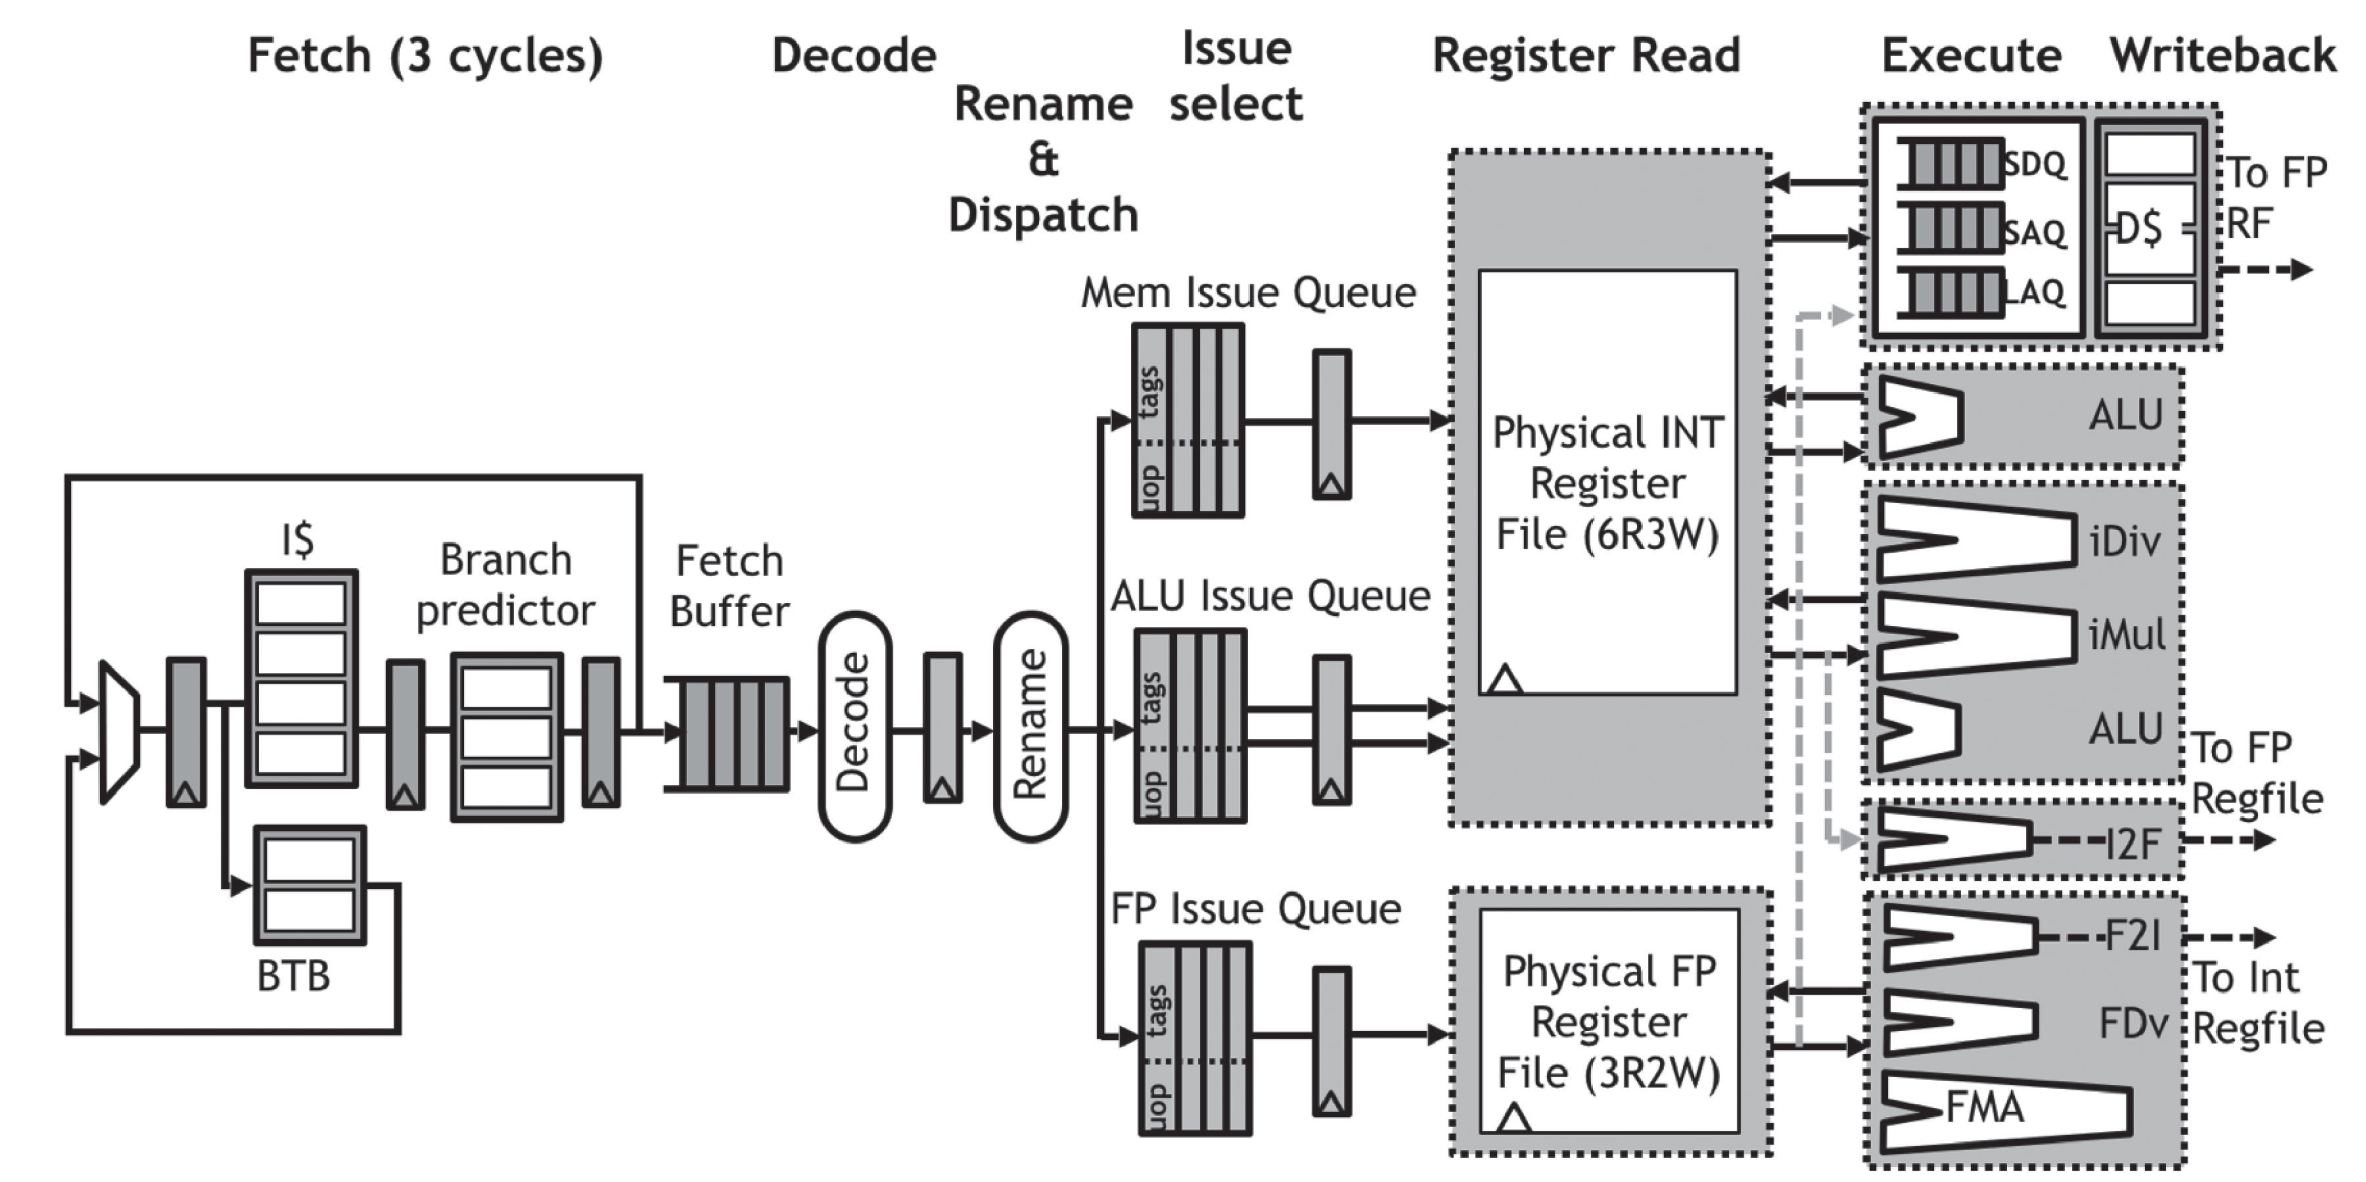
\includegraphics[width=15cm]{../ooo/broom-pipeline}
};
\end{tikzpicture}
\imagecredit{Figure from Celio et al., ``BROOM: An Open Source Out-Of-Order Processor With Resilient Low-Voltage  Operation in 28-nm CMOS''}
\end{frame}


\subsection{data flow limit}
\usetikzlibrary{shapes}

\begin{frame}[fragile,label=dfLimit]{data flow model and limits}
    \begin{tikzpicture}
        \tikzset{
            var/.style={draw,rectangle,fill=blue!30},
            op/.style={draw,ellipse,fill=yellow!40},
            node distance=4mm,
        }
        \begin{scope}[
                start chain=going below,
                every join/.style={thick,-Latex},
                every node/.style={on chain,op},
            ]
            \node[var] (sn1) at (0,1) {sum};
            \node[join] (s0)  {+};
            \node[join] (s1) {+};
            \node[join] (s2) {+};
            \node[join] (s3) {+};
        \end{scope}
        \node[var,right=2cm of s3] (sumFinal) {sum (final)};
        \draw[thick,-Latex] (s3) -- (sumFinal);
        \begin{scope}[
                start chain=going below,
                every node/.style={on chain,op},
            ]
            \node (l0) at (2,1) {load};
            \node (l1) {load};
            \node (l2) {load};
            \node (l3) {load};
        \end{scope}
        \begin{scope}[
                start chain=going below,
                every join/.style={thick,-Latex},
                every node/.style={on chain,op,join},
            ]
            \node[var] (a0) at (4,2.2) {A + i};
            \node (a1) {+ 1};
            \node (a2) {+ 1};
            \node (a3) {+ 1};
        \end{scope}
        \begin{visibleenv}<all:4>
        \node[op] (c1) at (7,1) {> A + N?};
        \draw[thick,-Latex] (a0) -- (c1);
        \node[op] (c3) at (7,-3) {> A + N?};
        \draw[thick,-Latex] (a3) -- (c3);
        \end{visibleenv}
        \begin{scope}[thick,-Latex]
            \foreach \x in {0,1,2,3} {
                \draw (a\x) -- (l\x) -- (s\x);
            }
        \end{scope}
        \begin{visibleenv}<all:1>
            \node[anchor=west] at ([xshift=1cm,yshift=-.5cm]a2.east) {
\begin{lstlisting}[language=C,style=small]
for (int i = 0; i < N; i += K) {
    sum += A[i];
    sum += A[i+1];
    ...
}
\end{lstlisting}
};
        \end{visibleenv}
        \begin{visibleenv}<all:2>
            \node[align=left,anchor=west] at (5, -1) {
                each yellow box = instruction\\
                arrows = dependences\\
                instructions only executed when dependencies ready
            };
        \end{visibleenv}
        \begin{visibleenv}<all:3>
            \node[draw,very thick,red,fit=(s0) (l1) (a2),label={east:three ops/cycle (\myemph{if} each one cycle)}] {};
        \end{visibleenv}
        \begin{visibleenv}<all:4>
            \node[draw,very thick,red,fit=(s0) (s3)] {};
            \node[align=left,anchor=west] at (5, -1) {
                can only do sums one at a time
            };
        \end{visibleenv}
    \end{tikzpicture}
\end{frame}



    % FIXME: remove or explain free list
    % FIXME: possibly use or mention two register files instead of mappings?

\subsection{multiple accumulator transformation}
\usetikzlibrary{chains,fit,shapes}

\begin{frame}{better data-flow}
    \begin{tikzpicture}
        \tikzset{
            var/.style={draw,rectangle,fill=blue!30},
            op/.style={draw,ellipse,fill=yellow!40},
            node distance=5mm,
        }
        \begin{scope}[
                start chain=going below,
                every join/.style={thick,-Latex},
                every node/.style={on chain,op},
            ]
            \node[var] (sn1) at (0,1) {sum1};
            \node[join] (s0)  {+};
            \node[join] (s1) {+};
            \node[join] (s2) {+};
        \end{scope}

        \begin{scope}[
                start chain=going below,
                every join/.style={thick,-Latex},
                every node/.style={on chain,op},
            ]
            \node[var] (tn1) at (10,1) {sum2};
            \node[join] (t0) {+};
            \node[join] (t1) {+};
            \node[join] (t2) {+};
        \end{scope}
        \begin{scope}[
                start chain=going below,
                every node/.style={on chain,op},
            ]
            \node (l0) at (2,1) {load};
            \node (l1) {load};
            \node (l2) {load};
        \end{scope}
        \begin{scope}[
                start chain=going below,
                every node/.style={on chain,op},
            ]
            \node (m0) at (8,1) {load};
            \node (m1) {load};
            \node (m2) {load};
        \end{scope}
        \begin{scope}[
                start chain=going below,
                every join/.style={thick,-Latex},
                every node/.style={on chain,op,join},
            ]
            \node[var] (a0) at (4,2.2) {A + i};
            \node (a1) {+ 2};
            \node (a2) {+ 2};
        \end{scope}
        \begin{scope}[
                start chain=going below,
                every join/.style={thick,-Latex},
                every node/.style={on chain,op,join},
            ]
            \node[var] (b0) at (6,2.2) {A + i + 1};
            \node (b1) {+ 2};
            \node (b2) {+ 2};
        \end{scope}
        \node[op] (combine) at (5, -4) {+};
        \node[below=.2cm of combine,var] (final) {sum (final)};
        \begin{scope}[thick,-Latex]
            \foreach \x in {0,1,2} {
                \draw (a\x) -- (l\x) -- (s\x);
                \draw (b\x) -- (m\x) -- (t\x);
            }
            \draw (s2) -- (combine);
            \draw (t2) -- (combine);
            \draw (combine) -- (final);
        \end{scope}
        \begin{visibleenv}<2>
            \node[draw,red, ultra thick,fit=(a2) (s0) (b2) (t0),label={[red!70!black,font=\bfseries,align=center]south: 6 ops/time \\ two sum adds/time}] {};
        \end{visibleenv}
        \begin{visibleenv}<3>
            \node[draw,red, ultra thick,fit=(s0) (s2)] {};
            \node[draw,red, ultra thick,fit=(t0) (t2)] {};
            \node[draw,red, ultra thick,fit=(combine),label={[red!70!black,font=\bfseries,align=center]north:4 adds of time --- 7 adds}] {};
        \end{visibleenv}
    \end{tikzpicture}
\end{frame}



\end{document}
